\documentclass[12pt,a4paper,oneside,ngerman]{article}
\usepackage[ngerman]{babel}
\usepackage[utf8]{inputenc}
\usepackage[T1]{fontenc}
\usepackage[scaled]{helvet}


\renewcommand{\familydefault}{\sfdefault}

\usepackage{subcaption}
\usepackage{textcomp}
\usepackage{titlesec}

\usepackage[hidelinks]{hyperref} % Hyperlinks
\usepackage[onehalfspacing]{setspace} % 1,5facher Zeilenabstand

\usepackage[margin=2.8cm]{geometry}
\usepackage{color}
\definecolor{bisque}{rgb}{1.0, 0.89, 0.77}
\definecolor{mygreen}{rgb}{0,0.5,0}
\definecolor{mygray}{rgb}{0.7,0.7,0.7}
\definecolor{mymauve}{rgb}{0.58,0,0.82}

\usepackage[square,sort,comma,numbers]{natbib}

\usepackage{graphicx} 	
\usepackage{wrapfig}

\usepackage{hyphenat}
\hyphenation{TUM in-te-res-siert} % Eigene

%\usepackage{pdfpages}
\usepackage{enumitem}

\usepackage{amsmath}


\usepackage{siunitx}
\DeclareSIUnit\molar{\mole\per\cubic\deci\metre}
\DeclareSIUnit\Molar{M}
\DeclareSIUnit\ccm{ccm}


%\newcommand{\sectionbreak}{\clearpage}
%\newcommand\subsectionbreak{\ifnum\value{subsection}>1\clearpage\fi}
%\newcommand{\sectionbreak}{\clearpage}
%\titleformat{\chapter}[display]
%  {\normalfont\bfseries}{}{0pt}{\Huge}
%\renewcommand\thesubsection{\alph{subsection}}

\usepackage{fancyhdr}
\pagestyle{fancy}
\fancyhf{}
\fancyhead[c]{Lucas Perocco Moreira, Johann Brenner}
\fancyfoot[c]{\thepage}

	 

\begin{document}


\thispagestyle{empty}


    \title{\vspace{15mm}\centering
\includegraphics[width = 100mm]{img/tum_logo.eps}
		\\[3\baselineskip]
		\textbf{\Huge Praktikumsbericht 3D Druck für Bioelektronik und Biomedizinische Anwendungen}}
	
	\author{\vspace{10mm}Lucas Perocco Moreira\\Johann Brenner}
	\date{\vspace{15mm}{\small Sommersemester 2019}}
	\maketitle
    \clearpage
    \tableofcontents
    \clearpage
    
    
    \section{Motivation}
    Rapid Prototyping von Strukturen mittels 3D-Druck ist essentiell für die Entwicklung von Mikro- und Nanotechnologie, denn die Einfachheit des Computer-gestützten Designs (CAD) und der additive Herstellungsprozess bergen viele Vorteile im Vergleich zu herkömmlichen Methoden wie Fotolithografie oder Fräsen - beispielsweise die verkürzte Design- und Herstellungszeit, der geringere Materialverbrauch und die Möglichkeit verschiedene Materialien in einem Bauteil zu verwenden.\cite{Vaezi2012,Chu2014}
Durch Forschung an biokompatiblen Materialien und in der Nanopartikeltechnologie, können nun auch elektronische Sensoren und medizinische Prothesen kostengünstig hergestellt werden.\cite{SanchezRomaguera2008,Mohammed2017}
Im Gegensatz zu herkömmlichen Druckern, konnten mit den in diesem Praktikum verwendeten Methoden Leiterbahnen für elektrochemische Sensoren und biokompatible Polymere in Mikrometer-Auflösung gedruckt werden.\cite{Skript}
Ziel des Praktikums war es, das Auflösungsvermögen eines Stereolithografen zu charakterisieren und dessen Prozessprotokoll für den Bau von Flusssensoren in einer Mikrofluidik zu optimieren. Aufgrund von Streueffekten im Harz und an der reflektierenden Oberfläche des Druck-Halters wird vermutet, dass auch an Stellen neben den belichteten Pixel polymerisiert wird. Nach den Drucken sollten somit minimale Öffnungsbreiten oder Durchmesser analysiert werden.
Für Passivierungsdrucke direkt auf Substraten wird getestet, wie optimal diese auf den Substraten bonden und ob sich auf den Öffnungen ein Mikrofilm bildet. Im Falle geschlossener Elektroden soll hier ein Nachätzen der Elektroden mit Schwefelsäure getestet werden. Zudem sollten die verwendeten Sensoren mittels Elektrochemischer Impedanzspektroskopie (EIS) bzw. Cyclovoltammetrie (CV) charakterisiert werden. Ein weiteres Ziel des Praktikum war es, mittels Inkjet-Printing drei-dimensionale Elektrodenstrukturen für den Aufbau eines Zellkultursensor-Systems zu drucken, welches aufgrund technischer Probleme nach zwei Prozessschritten eingestellt wurde.
    
    \clearpage
    \section{Theoretische Grundlagen}
    \subsection{Stereolithographie}

Stereolithographisches (SLA) 3D-Drucken kreiert feste dreidimensionale Objekte Schicht für Schicht mittels additiver Fertigungstechnik. Dabei wird ein Halter, auf welchem die Struktur gedruckt wird, in ein mit Harz gefülltes Reservoir eingetaucht und Schicht für Schicht angehoben. Anfangs taucht der Halter bis zum Boden, hebt sich dann um eine Schichthöhe und nun wird die erste Schicht belichtet, wobei die Belichtung das Harz polymerisiert und aushärtet. Für die nächste Schicht fährt der Halter wieder eine Schicht höher und die nächste wird belichtet, welche auch mit der ersten Schicht polymerisiert und so tatsächlich auch eine chemische Verbindung hergestellt wird, anders zu sog. Fused-Deposition-Modeling (FDM) Drucker, die die einzelnen Schichten nur physikalisch bzw. thermisch miteinander verbinden.

\subsection{Tintenstrahldrucken}

Ein Tintenstrahl oder Inkjet Drucker druckt sowohl zweidimensionale als auch dreidimensionale Strukturen, jedoch in kleineren Auflösungen verglichen mit dem SL-Drucker. Zudem können hier mit unterschiedlichen Tinten gedruckt werden, die beispielsweise leitfähig oder wasserlöslich sein können. Die Flüssigkeit im Tintenreservoir wird mit Hilfe eines piezoelektrischen Wandlers angeregt, sodass aus einer sehr schmalen Düse einzelne Tropfen mit Volumen von wenigen \si{\pico\liter} herausschießen, auf dem Substrat auftreffen und dort Punkte bilden. Mit geschickter Ansteuerung des Druckkopfs und Überlagerung der einzelnen Punkte können dreidimensionale Strukturen erzeugt werden.

    
    \clearpage
    \section{Material und Methoden}
    
\subsection{Stereolithografisches Drucken}

Zunächst sollen die Grenzen bzgl. lateraler und vertikaler Auflösung eines Stereolithographen (50X, Miicraft) mit einer Pixelauflösung von 30 µm erfasst werden. Dazu werden verschiedene sowohl Single- als auch Multilayer Strukturen gedruckt.

\subsubsection{Preparation des CAD Models}

Mit einer Pixelauflösung des Druckers von \SI{30}{\micro\meter} wurden die Strukturen so modelliert, dass diese an einem \SI{30}{\micro\meter} x \SI{30}{\micro\meter} Raster ausgerichtet sind, damit später beim Druckauftrag der Slicer an die Wänden der Kanäle volle Pixel und im Kanal nicht belichtet. Bei einem Misalignment wird der Kanal teilweise belichtet, somit auch mitpolymerisiert und es bildet sich im Kanal eine feste Struktur, die vermieden werden soll.

\paragraph{Axondioden\\}


\begin{wrapfigure}[11]{r}{.4\textwidth}
\vspace{5pt}
\centering
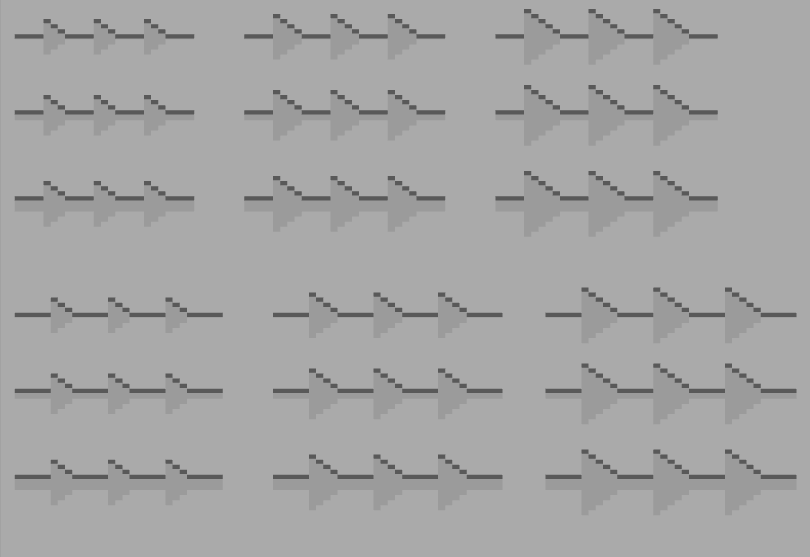
\includegraphics[width=\linewidth]{img/AxonDiode.png}
\caption{Modellierte, pixelausgerichtete Axon-Guiding Strukturen}
\label{fig:AxonDiode}
\end{wrapfigure}

Axondioden werden für Nachbildung von unidirektionalen, synaptischen Verbindungen gebraucht. Hier werden Dreiecke hintereinander gesetzt und mit einem dünnen Kanal verbunden. Dies ist in nebenstehender Abbildung zu erkennen.

Die Dreiecke sorgen dafür, dass nur die Source-Axone von der Hypothenuse des ersten Dreiecks mit Hilfe der beide Katheten wieder zum Kanal und das bis zum Kanal des letzten Dreiecks zum Ziel-Axon schafft. Aus Sicht des Ziel-Axons wird es durch die auseinander laufenden Katheten daran gehindert die Kanäle zu durchlaufen und beim Source-Axon anzukommen.\cite{Gladkov2017}

\paragraph{Wells\\}

Wells sind für Elektroden vorgesehen. Da diese bei rechteckigem Design an den Ecken nicht gut genug belichtet werden und daher eher rund ausfallen, wird außerhalb des Quadrats an jeder Ecke ein weiteres Pixel hinzugefügt, welches mitbelichtet wird und die Struktur letztendlich keine runden Ecken enthält.  

\paragraph{Kanäle\\}

Die Strukturen aus Inventor und Fusion werden dann in Fusion zu einer Datei zusammengeführt und auf eine 3 mm dicke Basis platziert. Es werden Strukturgruppen in vier unterschiedlichen Höhen gedruckt: 10 µm, 25 µm, 50 µm und 100 µm. Die Datei wird darauf als .stl-Datei exportiert und kann an den Drucker weitergegeben werden.

Um die maximale Auflösung des Druckers zu analysieren werden aufgrund der vom Hersteller angegebenen lateralen Auflösung von 30 µm, alle Strukturen in Vielfachen von 30µm-Pixeln realisiert. Bei einer Struktur wird versucht, einen 15 µm breiten Kanal zu konstruieren, indem zwei 30µm-Pixelreihen teilweise belichtet werden und sich in der Mitte der beiden ein dünner Kanal bildet. So werden Kanalbreiten von 30 µm bis 150 µm in 30 µm Schritten erstellt. Auch um 45° gedrehte Kanäle werden gedruckt, um schräge Strukturen zu analysieren. \\

Es soll nicht nur die Auflösung des Druckers erfasst werden, sondern auch welche Layerhöhen verlässlich möglich sind, beispielsweise ob eine 100 µm hohe Struktur besser mit zehn mal 10 µm Layer, vier mal 25 µm oder ein mal 100 µm Layer gedruckt wird und auch, ob eine 10 µm hohe Struktur überhaupt Kanäle frei druckt.

\subsubsection{Durchführung}

Zunächst wird das Reservoir des Druckers mit einem Harz (MedicalPrintClear (MPC) oder eigens gemischter Poly(ethylenglycol) diacrylat (PEGDA) - Lösung) befüllt. PEGDA-Lösung wird mit \SI{2}{\percent} Fotoinitiator Omnirad 2100 (IGM), \SI{0.1}{\percent} UV-absorbierender 5-Benzoyl-4-hydroxy-2-methoxybenzolsulfonsäure (HMBS, Sigma) und \SI{0.01}{\percent} Oxidationsmittel 2,2,6,6-Tetramethylpiperidinyloxyl (TEMPO, Sigma) in PEGDA (mittlere Molmasse 250, Sigma) in einem Ultraschallbad (VWR) gemischt. Die .stl-Datei wird in der Miicraft Software gesliced und mit den gewünschten Druckeinstellungen in eine Mii-Datei konvertiert, die letztendlich zum Druck aufgegeben wird. Die verwendeten Druckeinstellungen waren hierbei (außer anders spezifiziert) \SI{125}{\percent} Leistung und \SI{1}{s} Exposurezeit für Standardlagen, sowie eine Basislage bei einer Exposurezeit von \SI{3}{s}. 

Nach der Fertigstellung wurde ein Skalpell verwendet, um den Druck von dem Picker zu entfernen. Anschließend wurde das gedruckte Objekt mit Isopropanol (99\%, Sigma) abgespritzt und für Zeiten von 5, 10 oder 30 Minuten in Isopropanol in einem Ultraschallbad gereinigt. Am Ende des Prozesses wurde der Druck mit Pressluft getrocknet und in einem Polymerisationsgerät (Otoflash G171) mit 2000 Blitzen unter einer Schutzgasatmosphäre aus Stickstoff ausgehärtet. Dieses strahlt im Wellenlängenbereich von 280 nm - 580 nm mit einer Leistung von 200 Watt. Mit 10 Blitzen pro Sekunde ergibt sich somit eine Belichtungszeit von 3 Minunten und 20 Sekunden bei einer Leistung von 200 W, also idealerweise einer Energie von 11,1 Wh. Optional kann der Druck anschließend im Ofen bei 40°C getrocknet werden, um die restlichen Lösungsmittel aus dem Druck zu verdunsten.


\subsubsection{Oberflächenvermessung}

Für die Oberflächenvermessung der gedruckten Objekte wurde ein konfokales Laser-Mikroskop (Profilometer VK-X 200, Keyence) genutzt. Dazu wurden Bilder optisch und mit dem Laserprofilometer in vorgegebenen Fokuslimits aufgenommen und aneinander gestitcht, um den gesamten Druck später vermessen zu können. Anschließend wurden mittels des Multi-File Analyzers (Keyence) standardisierte, manuelle Messungen von Profiltiefen, teils mit einem Durchschnitt von 5-20 Linien durchgeführt. Das Standardprotokoll bestand sich zum Einen aus der Vermessung aller Kanalstrukturen mittels einer Linie senkrecht zum Kanal mit einem Durchschnitt aus 20 Linien. Zum Anderen wurden die Wells mit verschiedenen Linien angepasst auf deren Größe vermessen (\SI{30}{\micro\meter}: 1 Linie, \SI{60}{\micro\meter}: 2 Linien, ab \SI{90}{\micro\meter}: 5 Linien).

\subsubsection{Silanisierung der Objektträger und Sensoren}

Damit MPC oder PEGDA besser am bzw. überhaupt erst am Objektträger oder Chips hielt, mussten diese zunächst silanisiert werden. Das Silanisierungsprotokoll lief wie folgt ab: \\
\\
1. Ultraschall in purem Toluol für \SI{5}{\minute}; Behälter mit Parafilm verschließen, um Verdunstung zu vermeiden\\
2. Plasmaaktivierung bei \SI{0.8}{\milli\bar} O$_2$ und 100 \% Leistung für \SI{5}{\minute} \\
3. Inkubation im Silan-Lösung für einen Tag; Silan-Lösung wurde aus 5 \% 3-trimethoxysilylpropyl methacrylat (TMSPMA) in Toluol hergestellt; Behälter mit Parafilm verschließen, um Verdunstung zu vermeiden\\
4. Erneut Ultraschall in purem Toluol für 5 Minuten; Behälter mit Parafilm verschließen, um Verdunstung zu vermeiden\\
5. Mehrmals mit dH$_2$O abspülen; gegebenfalls kurz Ultraschall, bis sich weißer Film von Objektträgern löst \\
6. Trocknen mit Pressluft \\
7. Trocknen im Ofen bei 120°C für eine Stunde \\
8. Lagerung im Ofen bei 75°C

\clearpage

\subsubsection{Mikrofluidik}
Zum Design der Mikrofluidik wurden einige theoretische Betrachtungen unter verschiedenen Vereinfachungen getroffen. Verbindungen zwischen den einzelnen Komponenten wurden vernachlässigt und die Dimensionen als ideal angenommen. Als Schlauch wurden jeweils \SI{20}{\centi\meter} Tygon Tubing (Außen - \O{}: 1/16", Innen - \O{}: 1/32") verwendet. Die rechteckige Zu- und Ableitung besitzt jeweils Dimensionen (l x b x h) von \SI{3.7}{\milli\meter} x \SI{1.0}{\milli\meter} x \SI{300}{\micro\meter}. Der Messkanal über dem Sensor misst \SI{8}{\milli\meter} x  \SI{1.0}{\milli\meter} x \SI{300}{\micro\meter}.\\
  
So ergibt nach der Reynoldszahl über dem Flussratensensor mit der Dichte von Wasser $\rho$ = \SI{1000}{\kilo\gram\per\cubic\meter} und einer charakteristischen Kanalbreite $w$ von \SI{1}{\milli\meter} nach (\ref{eq:reynolds}) eine laminare Strömung für Geschwindigkeiten unter \SI{2.3}{\meter\per\second}

\begin{equation}
    \mathit{Re} = \frac{\rho \, v \, w}{\eta}\ <\ 2300 \label{eq:reynolds}
\end{equation}
  

Unter der Vernachlässigung sämtlicher kapazitiver Effekte ergibt sich ein Netzwerk aus rein seriellen Widerständen, für welche Formel (\ref{eq:ohm}) gilt.\cite{Kirby2009} In den folgenden Formel bezeichnen $l$, $w$, $h$ und $r$ jeweils die charakteristischen Dimensionen Länge, Breite, Höhe und Radius. Mit der Beschränkung auf Wasser als Medium ergibt sich die dynamische Viskosität $\eta$ zu \SI{1}{\milli\pascal\second}. Mit geeigneten Annahmen ($h$ < $w$) vereinfacht sich Gleichung (\ref{eq:rect_compl}) zu (\ref{eq:rec_easy}).\cite{TheoreticalMicrofluidics} Mit diesen Gleichungen ergeben sich also $R_{Schlauch}$ zu \SI{1.98e9}{\pascal\second\per\cubic\meter}, $R_{Kanal}$ zu \SI{4.38e9}{\pascal\second\per\cubic\meter} und $R_{Schlauch}$ zu \SI{2.03e9}{\pascal\second\per\cubic\meter}.
 \begin{align}
     Q\ &=\ \frac{\Delta p}{\sum\limits_{Fluss} R} \label{eq:ohm}\\
     \sum\limits_{Fluss} R\ &=\ R_{Schlauch}+ R_{Zulauf} +R_{Kanal} + R_{Ablauf} + R_{Schlauch}\\
     R_{Zulauf}\ &=\ R_{Ablauf} \\
     \sum\limits_{Fluss} R\ &=\ 2\ \cdot\ R_{Schlauch}\ +\ 2\ \cdot\ R_{Zulauf}\ +\ R_{Kanal}\\
     R_{Schlauch}\ &=\ \frac{8\eta l}{\pi r^4}\ =\ \frac{8\cdot\SI{1}{\milli\pascal\second} \cdot \SI{200}{\milli\meter}}{\pi \cdot \SI{1.58}{\milli\meter}^4}\ =\ \SI{8.17e7}{\pascal\second\per\cubic\meter} \\
     R_{Kanal, Zulauf}\ &=\ \frac{12 \eta l}{w\ h^3}\ \left[1-6 \left(\frac{h}{w}\right) \sum\limits_{n=0}^{\infty} \left( \frac{(2n+1)\pi}{2} \right)^{-5} \tanh{ \left( \frac{(2n+1)\pi\ w}{2\h} \right) } \right]^{-1} \label{eq:rect_compl}\\
     R_{Kanal, Zulauf}\ &\approx \frac{12 \eta l}{w h^3(1-(0.630h)/w)} \label{eq:rec_easy} 
 \end{align}
 Daher ergibt sich folgende Relation für die Flussrate abhängig vom angelegten Druck:
 \begin{equation}
     Q(\Delta p) = \frac{\Delta p}{\SI{1.10e10}{\pascal\second\per\cubic\meter}}
 \end{equation}
    \subsection{Inkjet Drucker}

\subsubsection{Vorbereitung der Polyvinylpyrrolidon-Silber-Nanopartikel}

Die Polyvinylpyrrolidon-Silber-Nanopartikel (PVP-AgNP) wurden mit einer 1ml-Spritze, durch einen Spritzenfilter (\SI{0.2}{\micro\meter}, Whataman) über eine Kanüle in die Druckerkartusche für den Inkjet-Drucker (CeraPrinter F-Series, CeraDrop) dispensiert. Die Kartusche wird mit einem Druckkopf mit 1pL-Düsen verbunden. Anschließend wurde für das Substrat die Folie aus Polyethylennaphthalat des Typs Q65HA auf die Größe A6 zugeschnitten, um die Druckplatte des Inkjet-Druckers zu bedecken. 

\subsubsection{Vorbereitung der Polyvinylpyrrolidon-Tinte}

Für die Vorbereitung der PVP-Tinte  wird ein 2:1 Gemisch von doppelt destilliertem Wasser und Triethylenglycol mit einem Gesamtvolumen von V$_{ges}$ = 3 ml hergestellt. Anschließend wird das PVP mit einer Masse von 5\% des V$_{ges}$, was einer Masse von 150 mg entspricht, mittels Feinwage eingewogen. Das PVP-Pulver in der Mischung wird durch einen Magnetrührer aufgelöst und auch hier wie bei der PVP-AgNP-Tinte in eine 1pL-Kartusche dispensiert.

\subsubsection{Inkjet Druck}

Für den Druck wird sowohl der Chuck als auch die Nozzle auf 30°C geheizt um Raumtemperaturschwankungen zu ignorieren, eine hohe Reproduzierbarkeit mit möglichst konstanten Eigenschaften zu erzielen und um Advektion beim Druck zu verhindern. Die zugeschnittene A6 Folie wird auf den Chuck gelegt und per Vakuum festgehalten. Nach Inspektion der 16 Nozzles mit Hilfe einer Kamera, ob 16 Droplets nebeneinander zu sehen sind, wird das Druck-Pattern und die Infill-Dichte der zu gedruckten Struktur analysiert, sodass der Druck aufgegeben werden kann. Nach dem Druck wird die Folie mit den gedruckten Strukturen in einem Ofen (Memmert) bei \SI{65}{\celsius} für mehrere Stunden getrocknet.

\subsubsection{Galvanisieren}

Da die Strukturen aus Silber-Nanopartikeln (AgNP) cytotoxisch sind, werden die Elektroden mit Gold beschichtet, um die Biokompabilität zu garantieren. Dafür werden auf die gedruckten Chips 300 µl einer Gold-Cyanid-Lösung (KAuCN$_2$) aufgetragen, die das komplexgebundene Gold für die Oberflächenbeschichtung enthält. In die Lösung wird  eine Referenzelektrode und eine Platinelektrode gelegt, die Gegenelektrode sind alle Silberstrukturen selbst, die über einen Sockel (IC51-390, Yamaichi) kurzgeschlossen und mit einer Krokodil-Klemme mit dem Potentiostat (VSP-300, BioLogic) verbunden sind. Für die Galvanisierung werden 12.000 Zyklen einer Pulsfolge durchgeführt. Der Puls besteht zunächst aus einer 20 ms langen Spannung von -0.9 V, gefolgt von 10 ms +0.4 V und abschließend 70 ms lang eine Spannung von 0 V. Somit dauert ein Zyklus 0.1 s, sodass ein kompletter Galvanisierungsprozess 20 Minuten benötigt. Die Pulsfolge ist in folgender Grafik abgebildet.
\begin{figure}
    \centering
    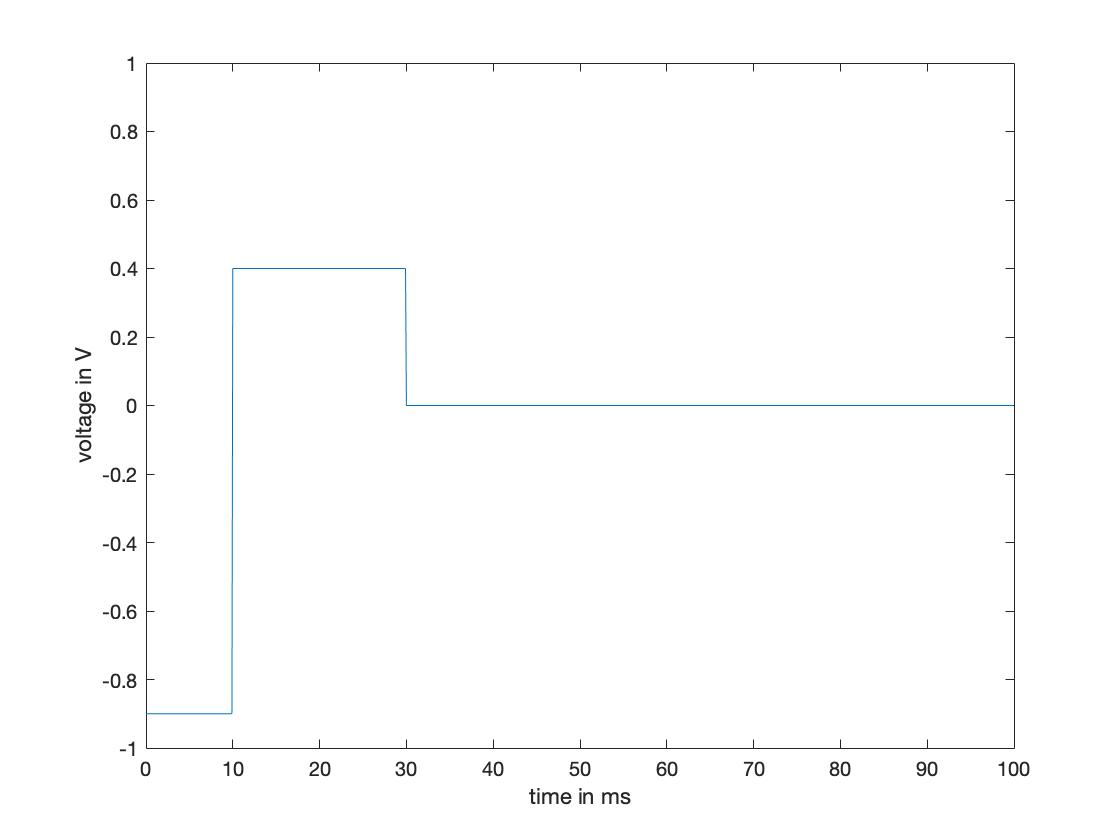
\includegraphics[width=1.0\textwidth]{img/galvanisierungpulsecurve.jpg}
    \caption{Charakteristischer Puls des Potentiostaten in einem Galvanisierungszyklus.}
    \label{fig:galvanisierung}
\end{figure}



\subsubsection{Aerosol Druck}
Um leitfähige, dreidimensionale Strukturen mittels Aerosol-Jetting zu drucken, wurde zuerst eine, auf Poly-3,4-ethylendioxythiophen polystyrolsulfonat (PEDOT:PSS) basierende, Lösung mit u.a. Carbon-Nano-Tubes (für eine verbesserte Leitfähigkeit) und Zellulose (für verbesserte mechanische Stabilität) versetzt. Nachdem Tinte und assemblierte Mechanik in den 3D-Drucker geladen waren, wurden die Drücke von Scherung, Absaugung und Atomisierung auf je \SI{600}{\ccm \per \minute}, \SI{615}{\ccm \per \minute} und \SI{15}{\ccm \per \minute} für einen kontinuierlichen, homogenen Tröpfchenstrom aus allen Nozzles geregelt.
\clearpage


    \subsection{Elektrochemische Methoden}
Soweit nicht anders spezifiziert, wurden die folgenden Parameter für das jeweilige Messverfahren verwendet. Die generierten Daten wurden mittels der PSTrace 5 (PalmSens) und MATLAB (MathWorks) Software analysiert und geplottet.
\subsubsection{Elektrochemische Impedanzspektroskopie}
Um die Durchlässigkeit des Passivierungslayers bzw. die Impedanz der einzelnen Elektroden zu bestimmen, wurde ein Impedanzspektrogramm mit einem Multiplex - Potentiostaten (Palmsens 3, PalmSens) erstellt. In diesem wurde in einem Bereich von \SIrange{0.1}{1e6}{Hz} mit einem Gleichanteil von \SI{0}{\volt}, sowie einem Wechselanteil von \SI{100}{\milli \volt} der resultierende Strom gegen eine Ag/AgCl Elektrode in einer Umgebungslösung von \SI{5}{\milli\Molar} Kaliumhexacyanidoferrat(III) (FeCy) in \SI{100}{\milli\Molar} Kaliumchlorid (KCl) Lösung in 41 Schritten gescannt. Für diese Messung wurde ein Sensorchip mit der unpassivierten Seite in einen Sockel (IC51-390, Yamaichi) eingespannt. Anschließend wurden \SI{500}{\micro\liter} der Standardlösung einpipettiert und die Referenz- bzw. Arbeitselektrode darin positioniert.

\subsubsection{Cyclovoltammetrie}
Die Messungen der CV gliederten sich in zwei Unterabschnitte. Zum Einen wurde die Sensitivität der Elektroden mittels CV vermessen, zum Anderen wurde CV genutzt, um während der Elektrodenreinigung mit Schwefelsäure eine Oxidation der Elektrodenoberfläche um einige Atomlagen zu erzeugen. Generell wurde die CV in einer Drei-Elektroden-Konfiguration gegen ein Ag/AgCl-Elektrode aufgenommen.
\paragraph{Sensitivitätscharakterisierung}
Für eine Sensitivitätscharakterisierung wurden zwei CV in \SI{5}{\milli\Molar} FeCy in \SI{100}{\milli\Molar} KCl-Lösung von \SIrange{-0.2}{0.6}{\volt} in \SI{10}{\milli\volt} Schritten und mit einer Scan-Rate von \SI{50}{\milli\volt\per\second} aufgenommen.
\paragraph{Reinigungs-CV}
Zur Reinigung der Elektroden in Schwefelsäure wurden diese (wiederum durch den Yamaichi-Sockel an den Potentiostaten angeschlossen) mit ca \SI{300}{\micro\liter} \SI{13}{\percent} H$_2$SO$_4$ (Schwefelsäure, Sigma) inkubiert und kurzgeschlossen. Während der Inkubation erzeugte man 40 CV-Hysteresen an allen (kurzgeschlossenen) Elektroden von \SIrange{-0.5}{1.5}{\volt} in \SI{10}{\milli\volt} Schritten mit einer Scan-Rate von \SI{500}{\milli\volt\per\second}. Schlussendlich wurde die Schwefelsäure mehrmals mit dH$_2$O von den Elektroden gewaschen.
    
    \clearpage
    \section{Ergebnisse}
    


% Grundlegendes "Story Telling":
% Herstellung eines Zellkultur-Sensor Systems für die Messung von Aktionspotentialen
% --> Inkjet printing
% --> Tintenpräparation
% --> Galvanisierung
% --> Aerosol-Jet für PDOT pillars
% --> Tintenpräparation
% --> Aufbau mit den 3 Druck Systemen in die Theorie
% Leider gebremst bzw Abgebrochen wegen Verbindungsproblemen aufgrund gebrochener Netzwerkkabel im Druckkopf 

% Etablierung eines optimalen Workflows für die Herstellung von Lennarts Flow-Rate-Sensor:
% Auflösung der Druckstrukturen für Kanal und Passivierung
% --> Keyence-Auswerung
% Entfernung des Mikrofilms für freie Elektroden 
% --> Folie 
% --> Messung vor/nach Behandlung mit Schwefelsäure
% Kanal mit Fittings Haftung von beidem aufeinander
% --> Haftung an den Seiten der Fittings offenbar zu gering
% Deswegen Kanal mit zylindrischen Inlets 200µm??? radial größer als Schlauchdurchmesser
% --> ?
% Bonding
% --> ? 
% Sensorperformance
% --> ? Kalibrierung, CV, Impedanz

\subsection{Druckerauflösung}
\subsubsection{Teststrukturen}
Um die Auflösungslimits des Stereolithografen zu evaluieren, wurden verschiedene Teststrukturen designt (Abb. \ref{fig:ResolutionV1}). Diese bestanden aus pixelausgerichteten Kanälen mit den Breiten \SIlist{15; 30; 60; 90; 120; 150}{\micro \meter}, Quadraten aus einem Vielfachen der Auflösung (\SI{30}{\micro\meter} x \SI{30}{\micro\meter}, \SI{60}{\micro\meter} x \SI{60}{\micro\meter},...,\SI{240}{\micro\meter} x \SI{240}{\micro\meter}), sowie denselben vorhergenannten Quadraten mit einem zusätzlichen Pixel diagonal an den äußeren Ecken.

\begin{figure}[!h]
    \centering
    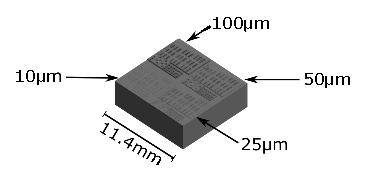
\includegraphics[width=\linewidth]{img/ResolutionV1.eps}
    \caption{Testdruck für die Auflösungsevaluation mit einem 2x2 Array derselben Struktur in den Layerhöhen \SI{10}{\micro\meter}, \SI{25}{\micro\meter}, \SI{50}{\micro\meter} und \SI{100}{\micro\meter} auf einem \SI{3}{\milli\meter} hohen Quader mit quadratischer Grundfläche (Kantenlänge \SI{11.4}{\milli\meter}).}
    \label{fig:ResolutionV1}
\end{figure}

Des Weiteren wurden verschiedene - ebenfalls pixelausgerichtete - Axondioden-Strukturen getestet. Bei solchen Kanälen wurden einerseits die Kanalbreite (\SIrange{1}{3}{px}) und -länge (\SIrange{3}{5}{px}) in den Durchgängen zwischen einzelnen Dioden und andererseits die Größe der dreieckigen Dioden (3-5 Stufen) variiert. Zu Testzwecken wurden außerdem um \SI{45}{\degree} gedrehte Kanäle, Quadrate und Wells in das Layout aufgenommen, jedoch aus Zeitgründen nicht ausgewertet.

Das fertig erstellte Layout wurde dann auf einem Quader mit den Maßen \SI{11.4}{\milli\meter} x \SI{11.4}{\milli\meter} x \SI{3}{\milli\meter} mit den Höhen \SI{10}{\micro\meter}, \SI{25}{\micro\meter}, \SI{50}{\micro\meter} und \SI{100}{\micro\meter} extrudiert. Dieses Werkstück diente nun als Standard für 3D-Drucke mit zwei verschiedenen Resins (MPC und PEGDA) auf den Slicerhöhen \SIlist{10; 25; 50; 100}{\micro\meter}.\\

Um die Druckbarkeit einer einlagigen Passivierungsschicht auf den Sensorchip mit definierter Öffnungsbreite und den zurückbleibenden Resin-Mikrofilm auf der Öffnung zu evaluieren, wurde eine zweite Teststruktur designt (Abb. \ref{fig:ResolutionLennart}). Hier wurden sowohl rechteckige Öffnungen verschiedener Breiten und Längen, als auch dieselben Öffnungen mit einer angeschlossenen Aufweitung auf beiden Seiten getestet. Diese Strukturen wurden einerseits pixelausgerichtet und anderseits um \SI{45}{\degree} gedreht mit \SI{10}{\micro\meter} und \SI{20}{\micro\meter} Höhe auf einen Mikroskopieträger gedruckt. Die Kanaldimensionen wurden mit folgenden Parametern designt:
\begin{itemize}
    \item \textbf{Breite:} \SIlist{30;60;90;120;150;210;300;510}{\micro\meter}
    \item \textbf{Länge:} \SIlist{300;600;900}{\micro\meter}
    \item \textbf{Endseiten:} Flache Enden, Endaufweitung mit Breite \SI{600}{\micro\meter} und Länge \SI{300}{\micro\meter}
\end{itemize}

\begin{figure}[!h]
    \centering
    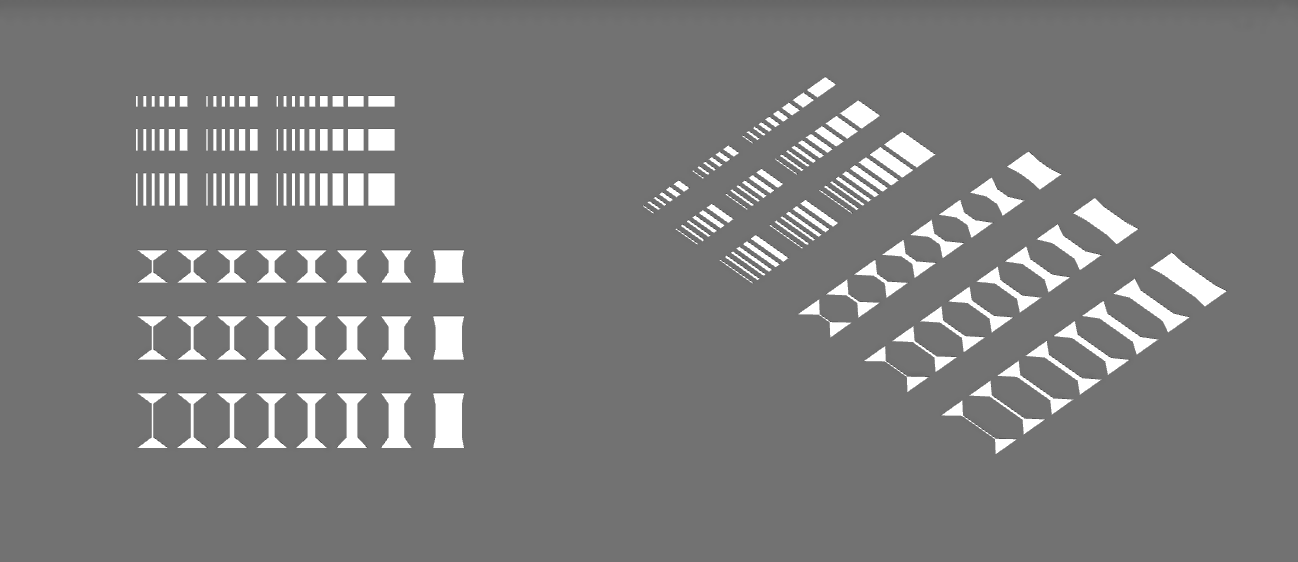
\includegraphics[width=\linewidth]{img/ResolutionLennart.png}
    \caption{Teststrukturen für die Bestimmung der Auflösung von Ein-Lagen-Drucken, sowie vorhandener Mikrofilme.}
    \label{fig:ResolutionLennart}
\end{figure}

\clearpage
\subsubsection{Auflösung}

\begin{figure}[!h]
    \centering
    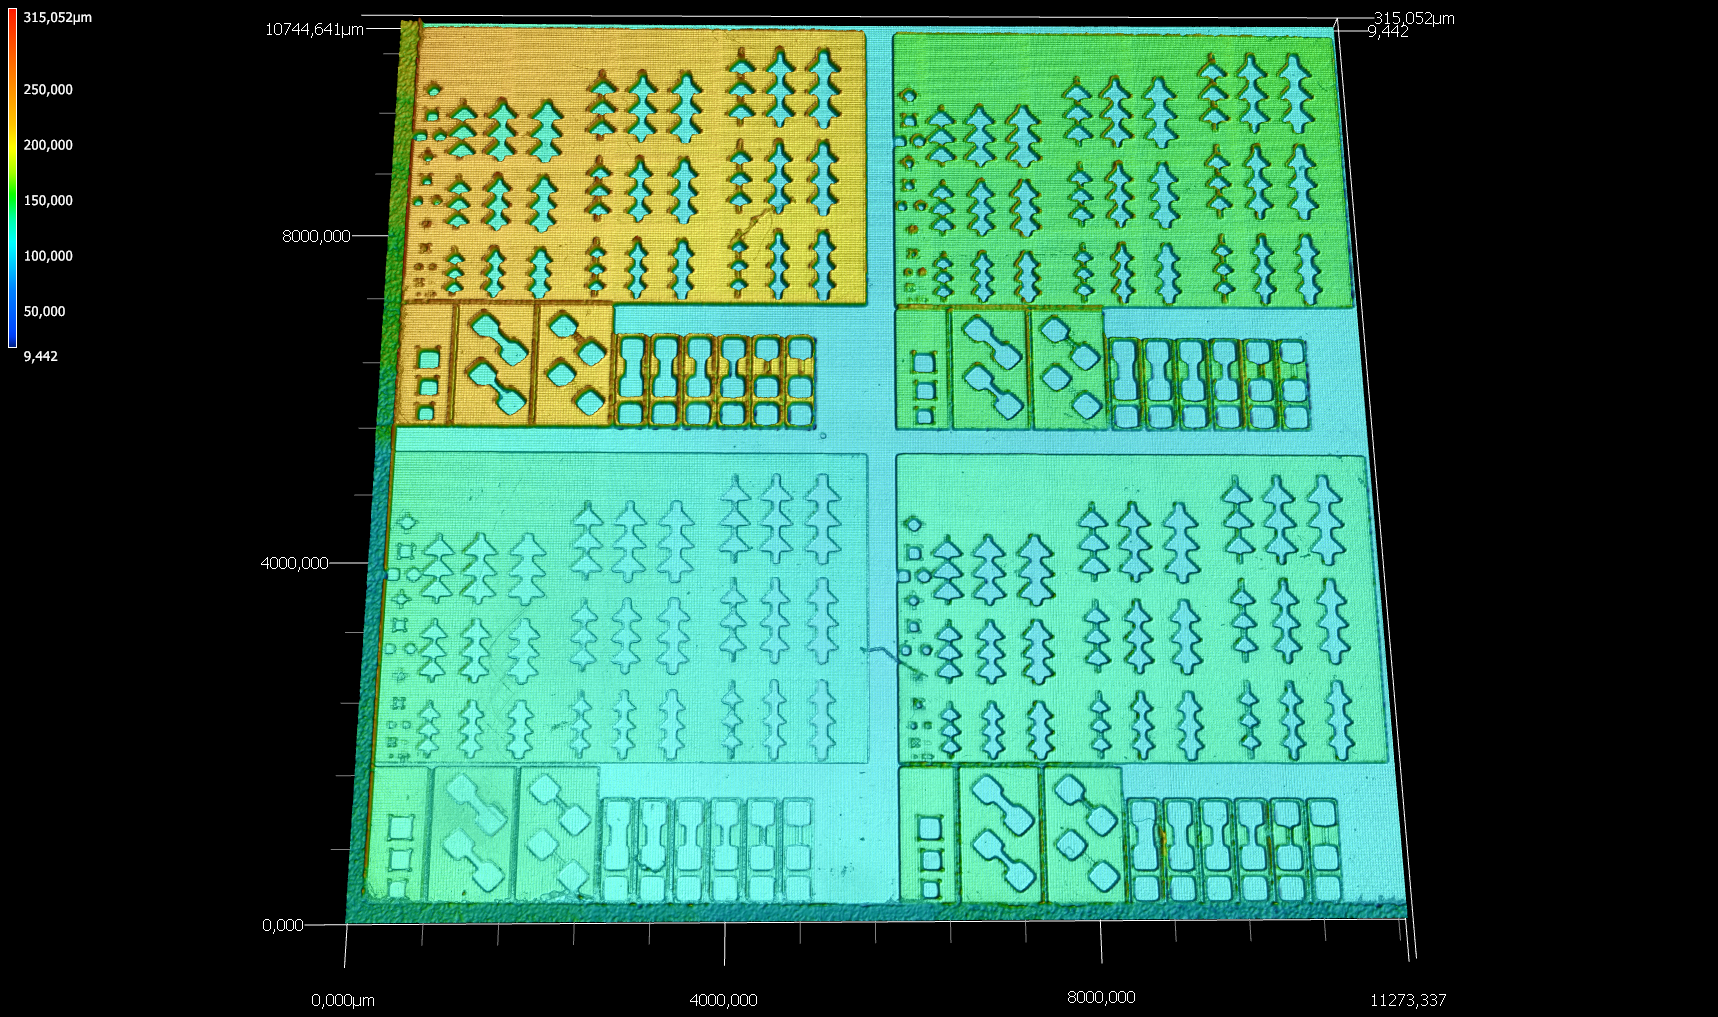
\includegraphics[width=\linewidth]{img/PEGDA-10um-3d.png}
    \caption{Oberflächenprofil des PEGDA Werkstücks mit \SI{10}{\micro\meter} z-Auflösung.}
    \label{fig:Surface_PEGDA_10um}
\end{figure}

Die Oberflächenvermessung der Testdrucke sollte nun die laterale und Tiefenauflösung des Druckers charakterisieren. Bereits vor der Durchführung bestand die Annahme, dass die höhere Viskosität des MPC gegenüber des PEGDA Resins die Auflösung negativ beeinflussen könnte, da mehr Material in den Strukturöffnungen diffusiv ausgehärtet würde.
Dies bestätigt ein Vergleich der Einzellagenstrukturen mit \SI{10}{\micro\meter} Höhe.

Der PEGDA-Druck (Abb. \ref{fig:PEGDA_10um}) zeigt eine im Durchschnitt höhere Tiefe als ursprünglich angepeilt. Das legt den Schluss nahe, dass zu wenig Resin in der Tiefe quervernetzt wird. Gleichzeit erhöht diese geringere Aushärtung die laterale Auflösung im Vergleich zu MPC. Diese Annahme wird qualitativ dadurch gestützt, dass die MPC Breiten konträr zum PEGDA zumeist unter der nominellen Breite liegen.

Im Gegensatz zum PEGDA-Druck fehlen bei MPC (Abb. \ref{fig:MPC_10um}) bereits die \SI{15}{\micro\meter} breiten Kanäle komplett und die Tiefen nähern sich erst ab \SI{150}{\micro\meter} Strukturbreite (also 5 Pixeln) den angepeilten \SI{10}{\micro\meter}. Dasselbe Bild ergibt sich für die ausgewerteten Höhen von \SIlist{25;50}{\micro\meter} unter Punkt \ref{appendix}. Zusätzlich sind bei den 3D-Profilometeraufnahmen der PEGDA-Drucke (im Gegensatz zu MPC) die Grenzen der einzelnen Mikrospiegel sichtbar.
Daraus kann man einerseits eine allgemein höhere Auflösung mit diesem Resin schließen, andererseits scheint eine homogene Oberfläche der Strukturen nicht gegeben zu sein. Wir vermuten, dass die Pixelkanten durch die Überlappung von aneinanderliegenden Linsen verursacht werden. \\
\clearpage
\begin{figure}[!h]
    \centering
    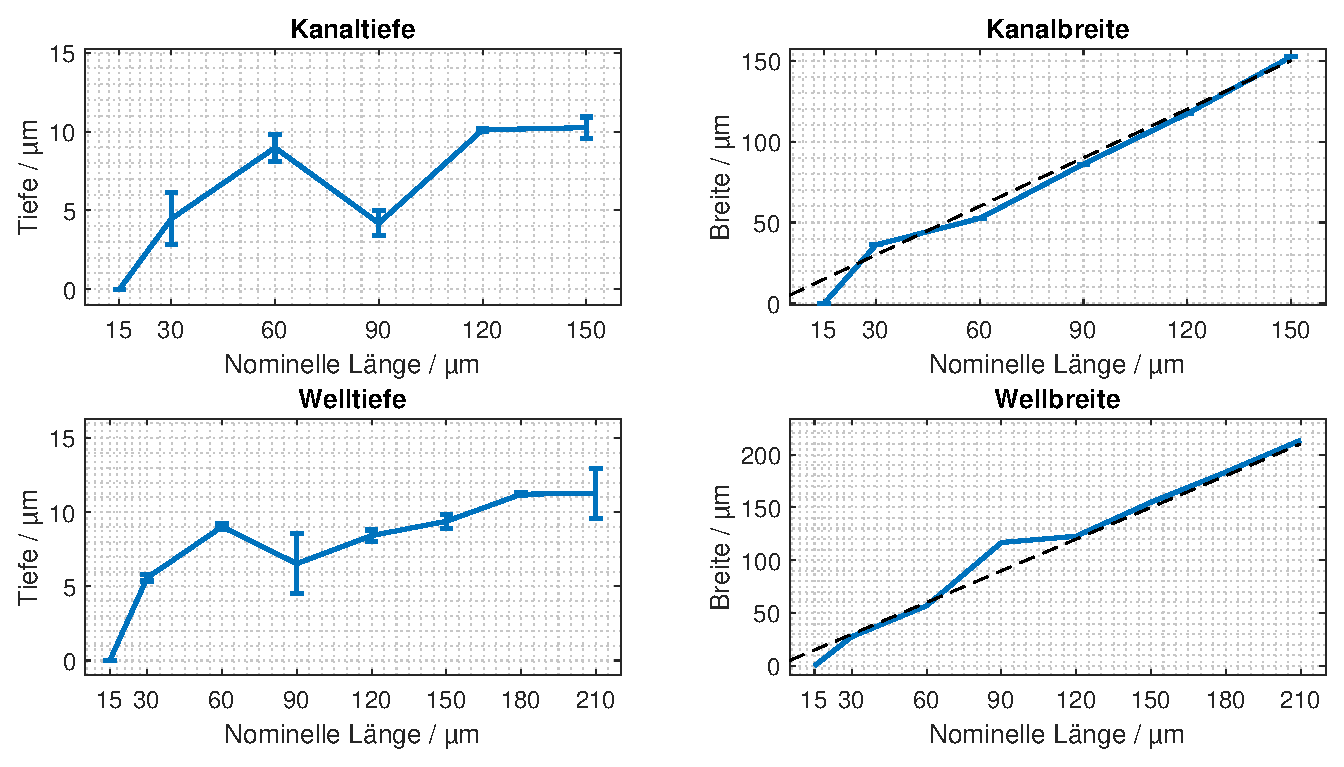
\includegraphics[width=\linewidth]{plot/10um_SL_ResolutionV1.eps}
    \caption{Profilometrie des \SI{10}{\micro\meter}-Einzellayers aus MPC. Da in den Kanalbreiten keine laterale Varianz messbar war (siehe Fehlerbalken Kanalbreite), wurden Fehlerbetrachtungen bei den Breitenprofilen vernachlässigt. (\textcolor{black}{\textbf{- - -}}) gibt die ideal gedruckte Breite an.}
    \label{fig:MPC_10um}
\end{figure}

\begin{figure}[!h]
    \centering
    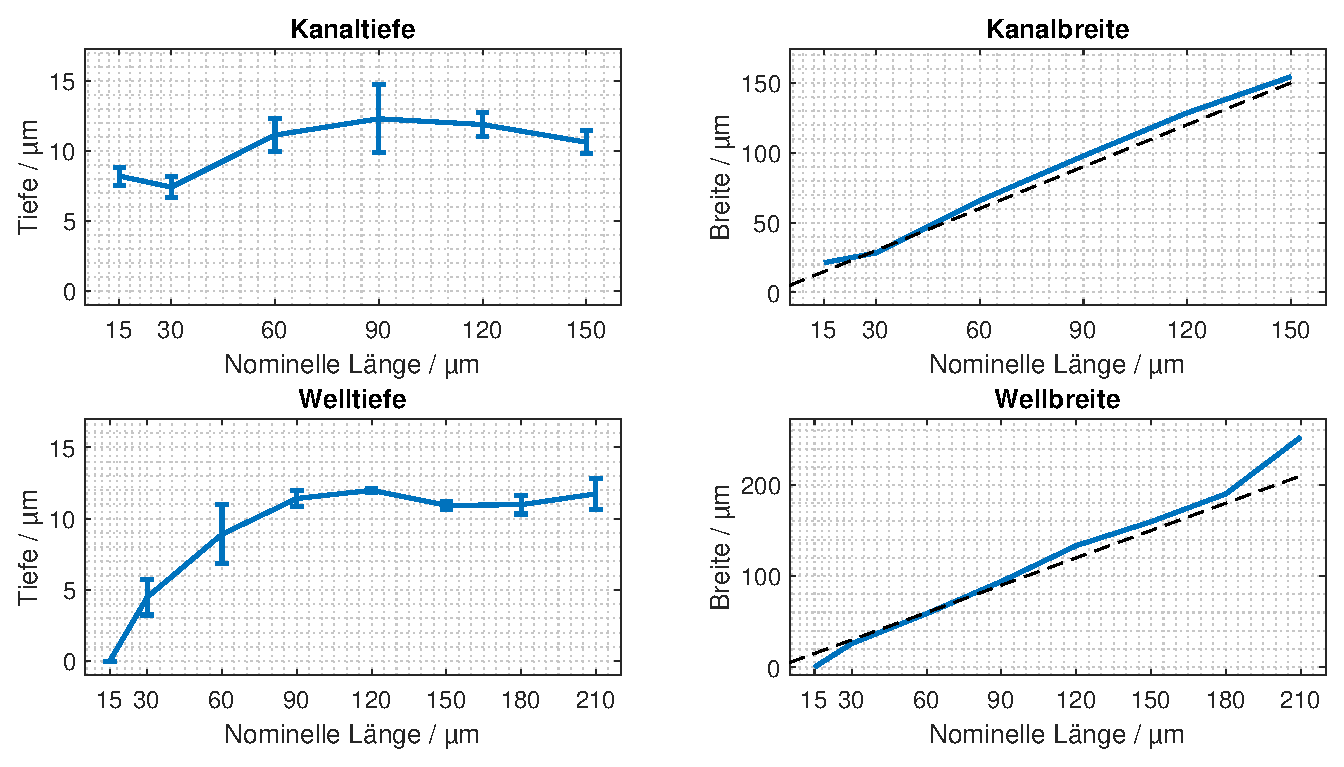
\includegraphics[width=\linewidth]{plot/PEGDA_10um_SL_ResolutionV1.eps}
    \caption{Profilometrie des \SI{10}{\micro\meter}-Einzellayers aus PEGDA. (\textcolor{black}{\textbf{- - -}}) gibt die ideal gedruckte Breite an.}
    \label{fig:PEGDA_10um}
\end{figure}
\clearpage

Als weiterer Punkt der Druckercharakterisierung wurde der Einflusses von Lichtintensität auf das Druckergebnis bestimmt. Aus Zeitgründen wurde hierbei die Leistung bei dem \SI{50}{\micro\meter}-Einzellayer der MPC-Drucke einmalig von \SI{125}{\percent} auf \SI{100}{\percent} - also um \SI{20}{\percent} - verringert. Die Exposurezeit von \SI{1}{\second} wurde konstant gehalten. Mit der verringerten Lichtleistung sollte dem diffusiven Quervernetzen des Resins an ungewollten Stellen entgegengewirkt werden.

Qualitativ kann man aus den Auswertungen von \SI{50}{\micro\meter} bei \SI{125}{\percent} (Abb. \ref{fig:MPC_50um}) und \SI{100}{\percent} (Abb. \ref{fig:MPC_50um_100perc}) erschließen, dass insbesondere \SIlist{15;30}{\micro\meter} Kanäle mit geringerer Leistung überhaupt erst aufgelöst werden können.

Aus ungeklärter Ursache sind die mit geringerer Leistung gedruckten Strukturen näher an der nominellen Tiefe von \SI{50}{\micro\meter}, als diejenigen der Standardleistung. Unseren bisherigen Ergebnissen nach, müssten im Druck mit höherer Energie durch erhöhte diffusive Strahlung mehr Resin quervernetzen und die Tiefe somit nachhaltig verringert werden.

\begin{figure}[!h]
    \centering
    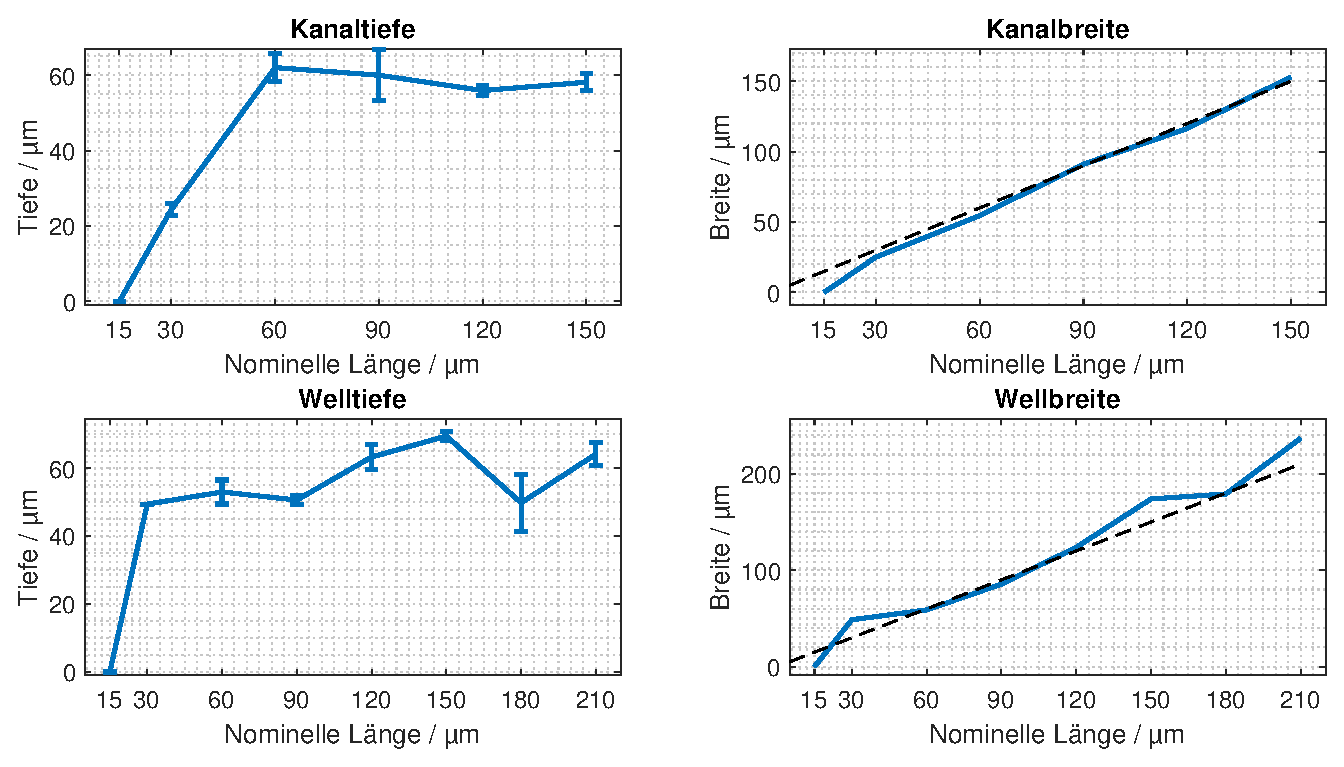
\includegraphics[width=\linewidth]{plot/50um_SL_ResolutionV1.eps}
    \caption{Profilometrie des \SI{50}{\micro\meter}-Einzellayers aus MPC. (\textcolor{black}{\textbf{- - -}}) gibt die ideal gedruckte Breite an.}
    \label{fig:MPC_50um}
\end{figure}
\clearpage
\begin{figure}[!h]
    \centering
    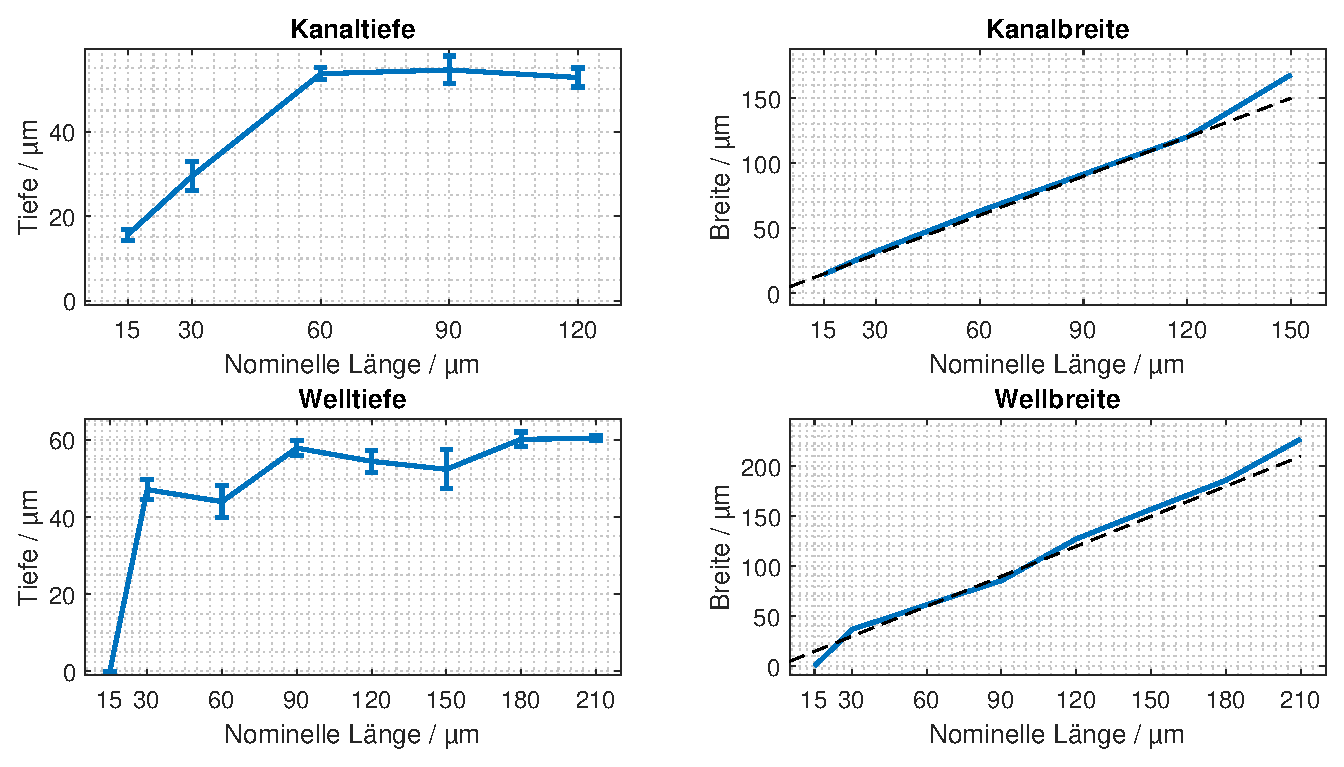
\includegraphics[width=\linewidth]{plot/50um_100perc_SL_ResolutionV1.eps}
    \caption{Profilometrie des \SI{50}{\micro\meter}-Einzellayers aus MPC mit \SI{100}{\percent} (also \SI{20}{\percent} weniger) Leistung.  (\textcolor{black}{\textbf{- - -}}) gibt die ideal gedruckte Breite an.}
   \label{fig:MPC_50um_100perc}
\end{figure}

\subsection{Passivierungsstrukturen}

Im Anschluss an die Auflösungstests, sollte eine auf einen silanisierten Glaschip gedruckte Passivierungsschicht des Druckers etabliert werden. Auf Basis der besseren Druckergebnisse des PEGDA Resins, wurden die folgenden Tests ausschließlich mit diesem Harz durchgeführt. In diesem Schritt sollte auf der einen Seite getestet werden, welche Öffnungsbreiten noch realisiert werden können. Auf der anderen Seite sollte die Vermutung eines Resin-Mikrofilms in der Öffnung bestätigt und entsprechende Gegenmaßnahmen ergriffen werden.

Zu diesem Zweck wurde zuerst eine Alignmentstruktur auf den Picker gedruckt, an dem der Glaschip später ausgerichtet werden sollte. Dieser wurde dann mittels Kapton auf dem gesäuberten Picker befestigt. Anschließend wurde die Passivierung mit einem Offset von \SI{0.52}{\milli\meter} auf den Chip gedruckt. Nach unterschiedlichen Behandlungsdauern mit Isopropanol in einem Ultraschallbad, wurden die Drucke dann im Profilometer vermessen. Dort zeigte sich, dass eine Behandlung von \SIlist{5;10;30}{\minute} bei Layerhöhen von \SIlist{10;20}{\micro\meter} keine Öffnung produzieren konnte.

Durch die Vorarbeiten anderer Studenten motiviert, wurde der Picker und die Alignmentstruktur mit einer schwarzen Mülltüte überklebt. Das Vorgehen basiert auf der Annahme, dass der graue Aluminiumpicker die Belichtung in das umliegende Resin zu stark reflektiert und es so mitaushärtet. Mit dem modifizierten Picker wurden die obigen Experimente noch einmal durchgeführt.

Die Ergebnisse nach verschiedenen Behandlungen (\SIlist{5;10;30}{\minute}) im Ultraschallbad sind in Abbildung \ref{fig:Microfilm} dargestellt. Hier sind bei größeren Strukturen deutliche Öffnungen sichtbar, sodass mit Vernachlässigung der kleinsten Öffnung minimale Parameter bestimmt werden können. Sowohl für die flachen, als auch für die aufgeweiteten Enden ergibt sich eine minimale Breite von \SI{240}{\micro\meter}. Die Länge der Öffnung scheint eine untergeordnete Rolle zu spielen und wurde in einem Bereich von \SIrange{300}{900}{\micro\meter} validiert.

Ein signifikanter Einfluss der aufgeweiteten Enden auf die Strukturöffnung gegenüber dem recheckigen Standard konnte nicht gezeigt werden. Auch scheint eine Verlängerung der Ultraschallbehandlung das Druckergebnis nicht zu verbessern. Im Gegenteil, bei schlechter Silanisierungsqualität bzw. allgemein schlechter Haftung des Drucks auf dem Glaschip löste sich in manchen Fällen die Passivierung wieder.

\begin{figure}[htb!]
\begin{subfigure}[l]{0.3\linewidth}
\centering
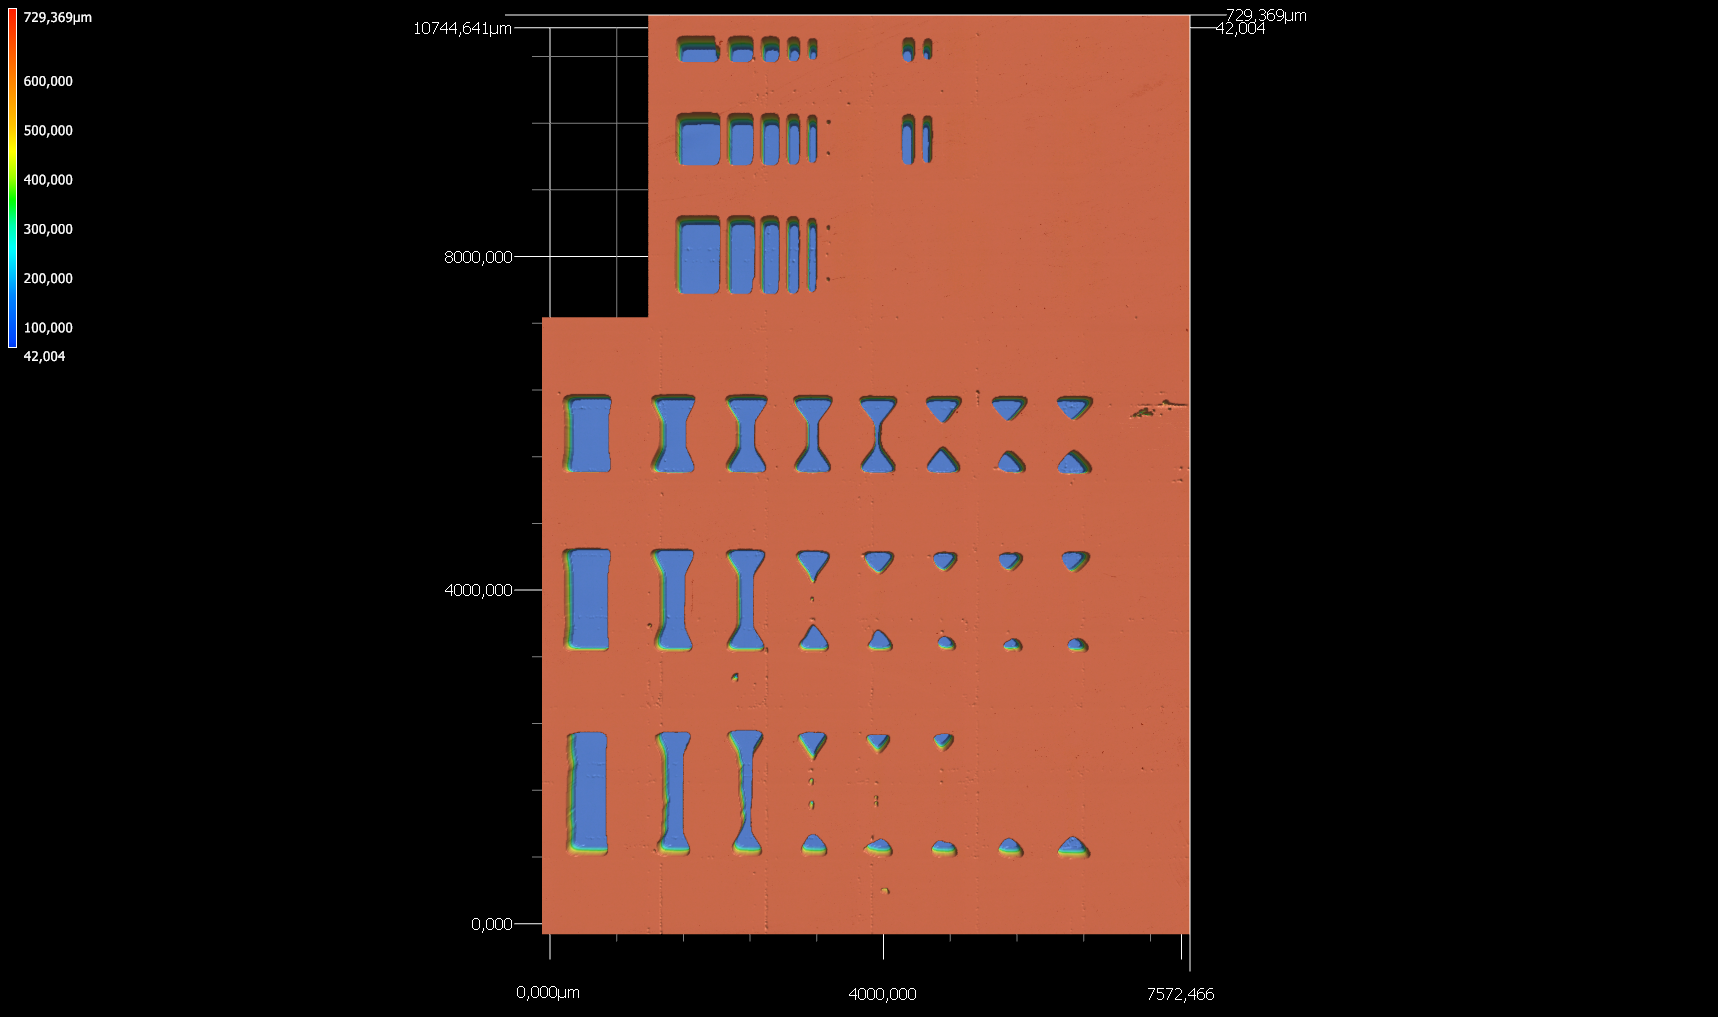
\includegraphics[clip, trim=0 0mm 50 0, width=\linewidth]{img/10um-05min-Folie-3d.png}
\subcaption{\SI{5}{\minute} Ultraschallbad}
\end{subfigure}%
\hspace{6mm}
\begin{subfigure}[c]{0.3\linewidth}
\centering
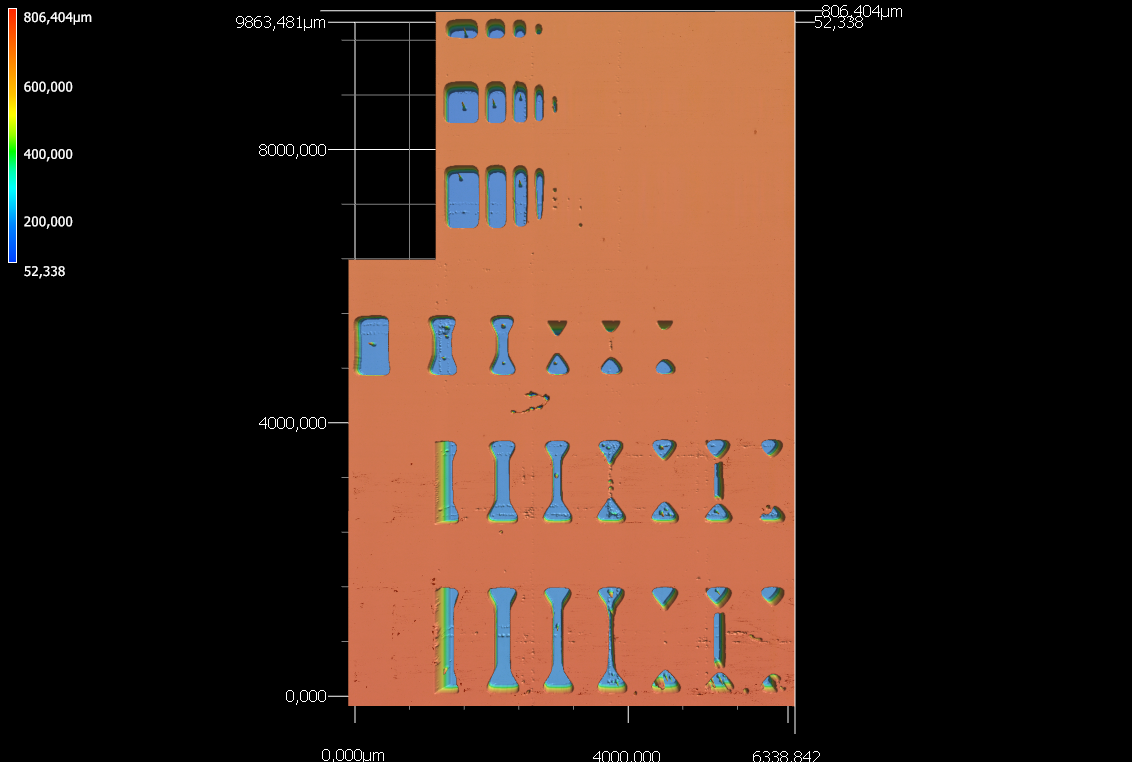
\includegraphics[clip, trim=0 0mm 0 0,width=\linewidth]{img/10um-10min-Folie-3d.png}
\subcaption{\SI{10}{\minute} Ultraschallbad}
\end{subfigure}%
\hspace{6mm}
\begin{subfigure}[r]{0.3\linewidth}
\centering
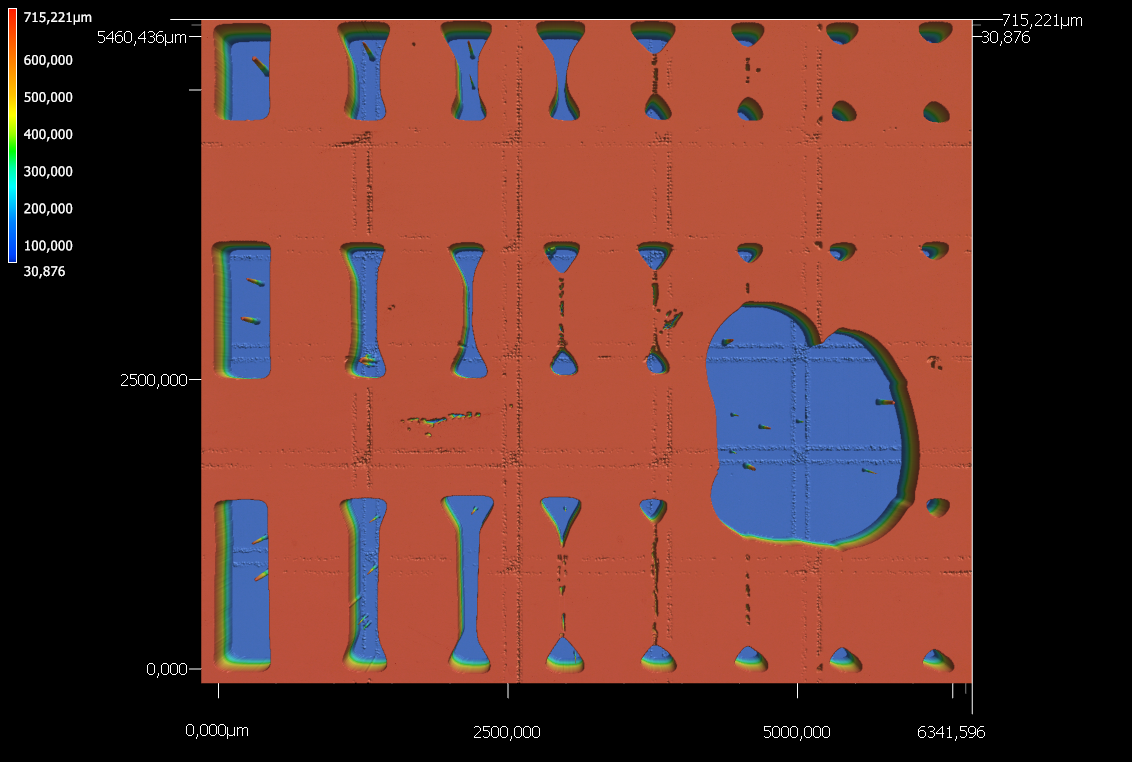
\includegraphics[clip, trim=0 0mm 0 0,width=\linewidth]{img/10um-30min-Folie-3d.png}
\subcaption{\SI{30}{\minute} Ultraschallbad}
\end{subfigure}
\caption{Oberflächen der \SI{10}{\micro\meter} passivierten Chips nach der Modifizierung des Pickers mit schwarzer Folie.}
\label{fig:Microfilm}
\end{figure}



\subsection{Bonding}

\begin{wrapfigure}[14]{r}{0.4\linewidth}
    \centering
    \vspace{-16pt}
    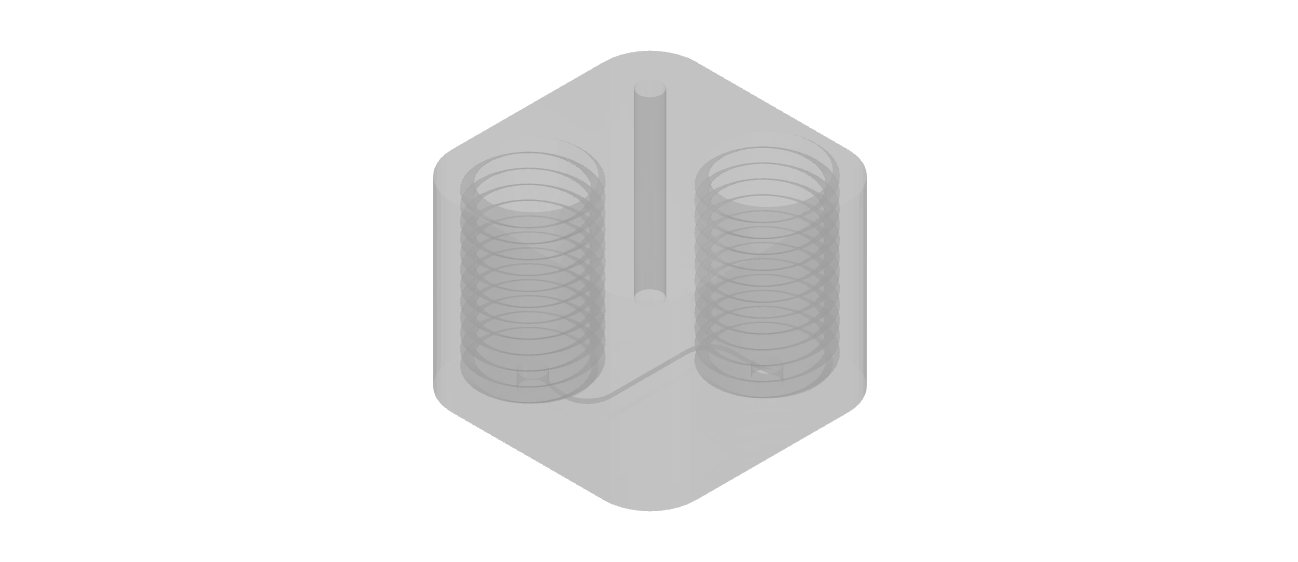
\includegraphics[clip,trim=11mm 2 10mm 3,width=1.15\linewidth] {img/Fitting.png}
    \caption{Mikrofluidikkanal mit 1/4\dq-28 Feingewinde für Fittings}
    \label{fig:Mikrofluidik_Gewinde}
\end{wrapfigure}
Als nächster Schritt im Workflow wurde die Verbindung von einer designten Mikrofluidik mit dem passivierten Sensorchip untersucht. Dafür wurden zuerst simple Kanäle mit Schraubverbindungen für Fittings der Elveflow- und Fluigent-Systeme designt (Abb. \ref{fig:Mikrofluidik_Gewinde}). Sowohl die Kanäle, als auch die passivierten Chips wurden vor dem Aushärten im Polymerisationsgerät in einer Schraubzwinge verpresst und so permanent verbunden.

In unseren Versuchen konnte in einem anschließenden Drucktest mit flüssigkeitsgefüllten Schläuchen keine Dichtigkeit nachgewiesen werden. Bei Drücken über \SI{20}{\milli\bar} trat an den Seiten der Inlets Flüssigkeit aus und der Kanal löste sich von der Passivierung. Bei zukünftigen Designs könnte ein zusätzlicher Abstand der Inlets zum Rand des Chips und somit mehr Klebefläche ein Lösungsansatz sein. \\

\begin{figure}[!ht]
    \centering
    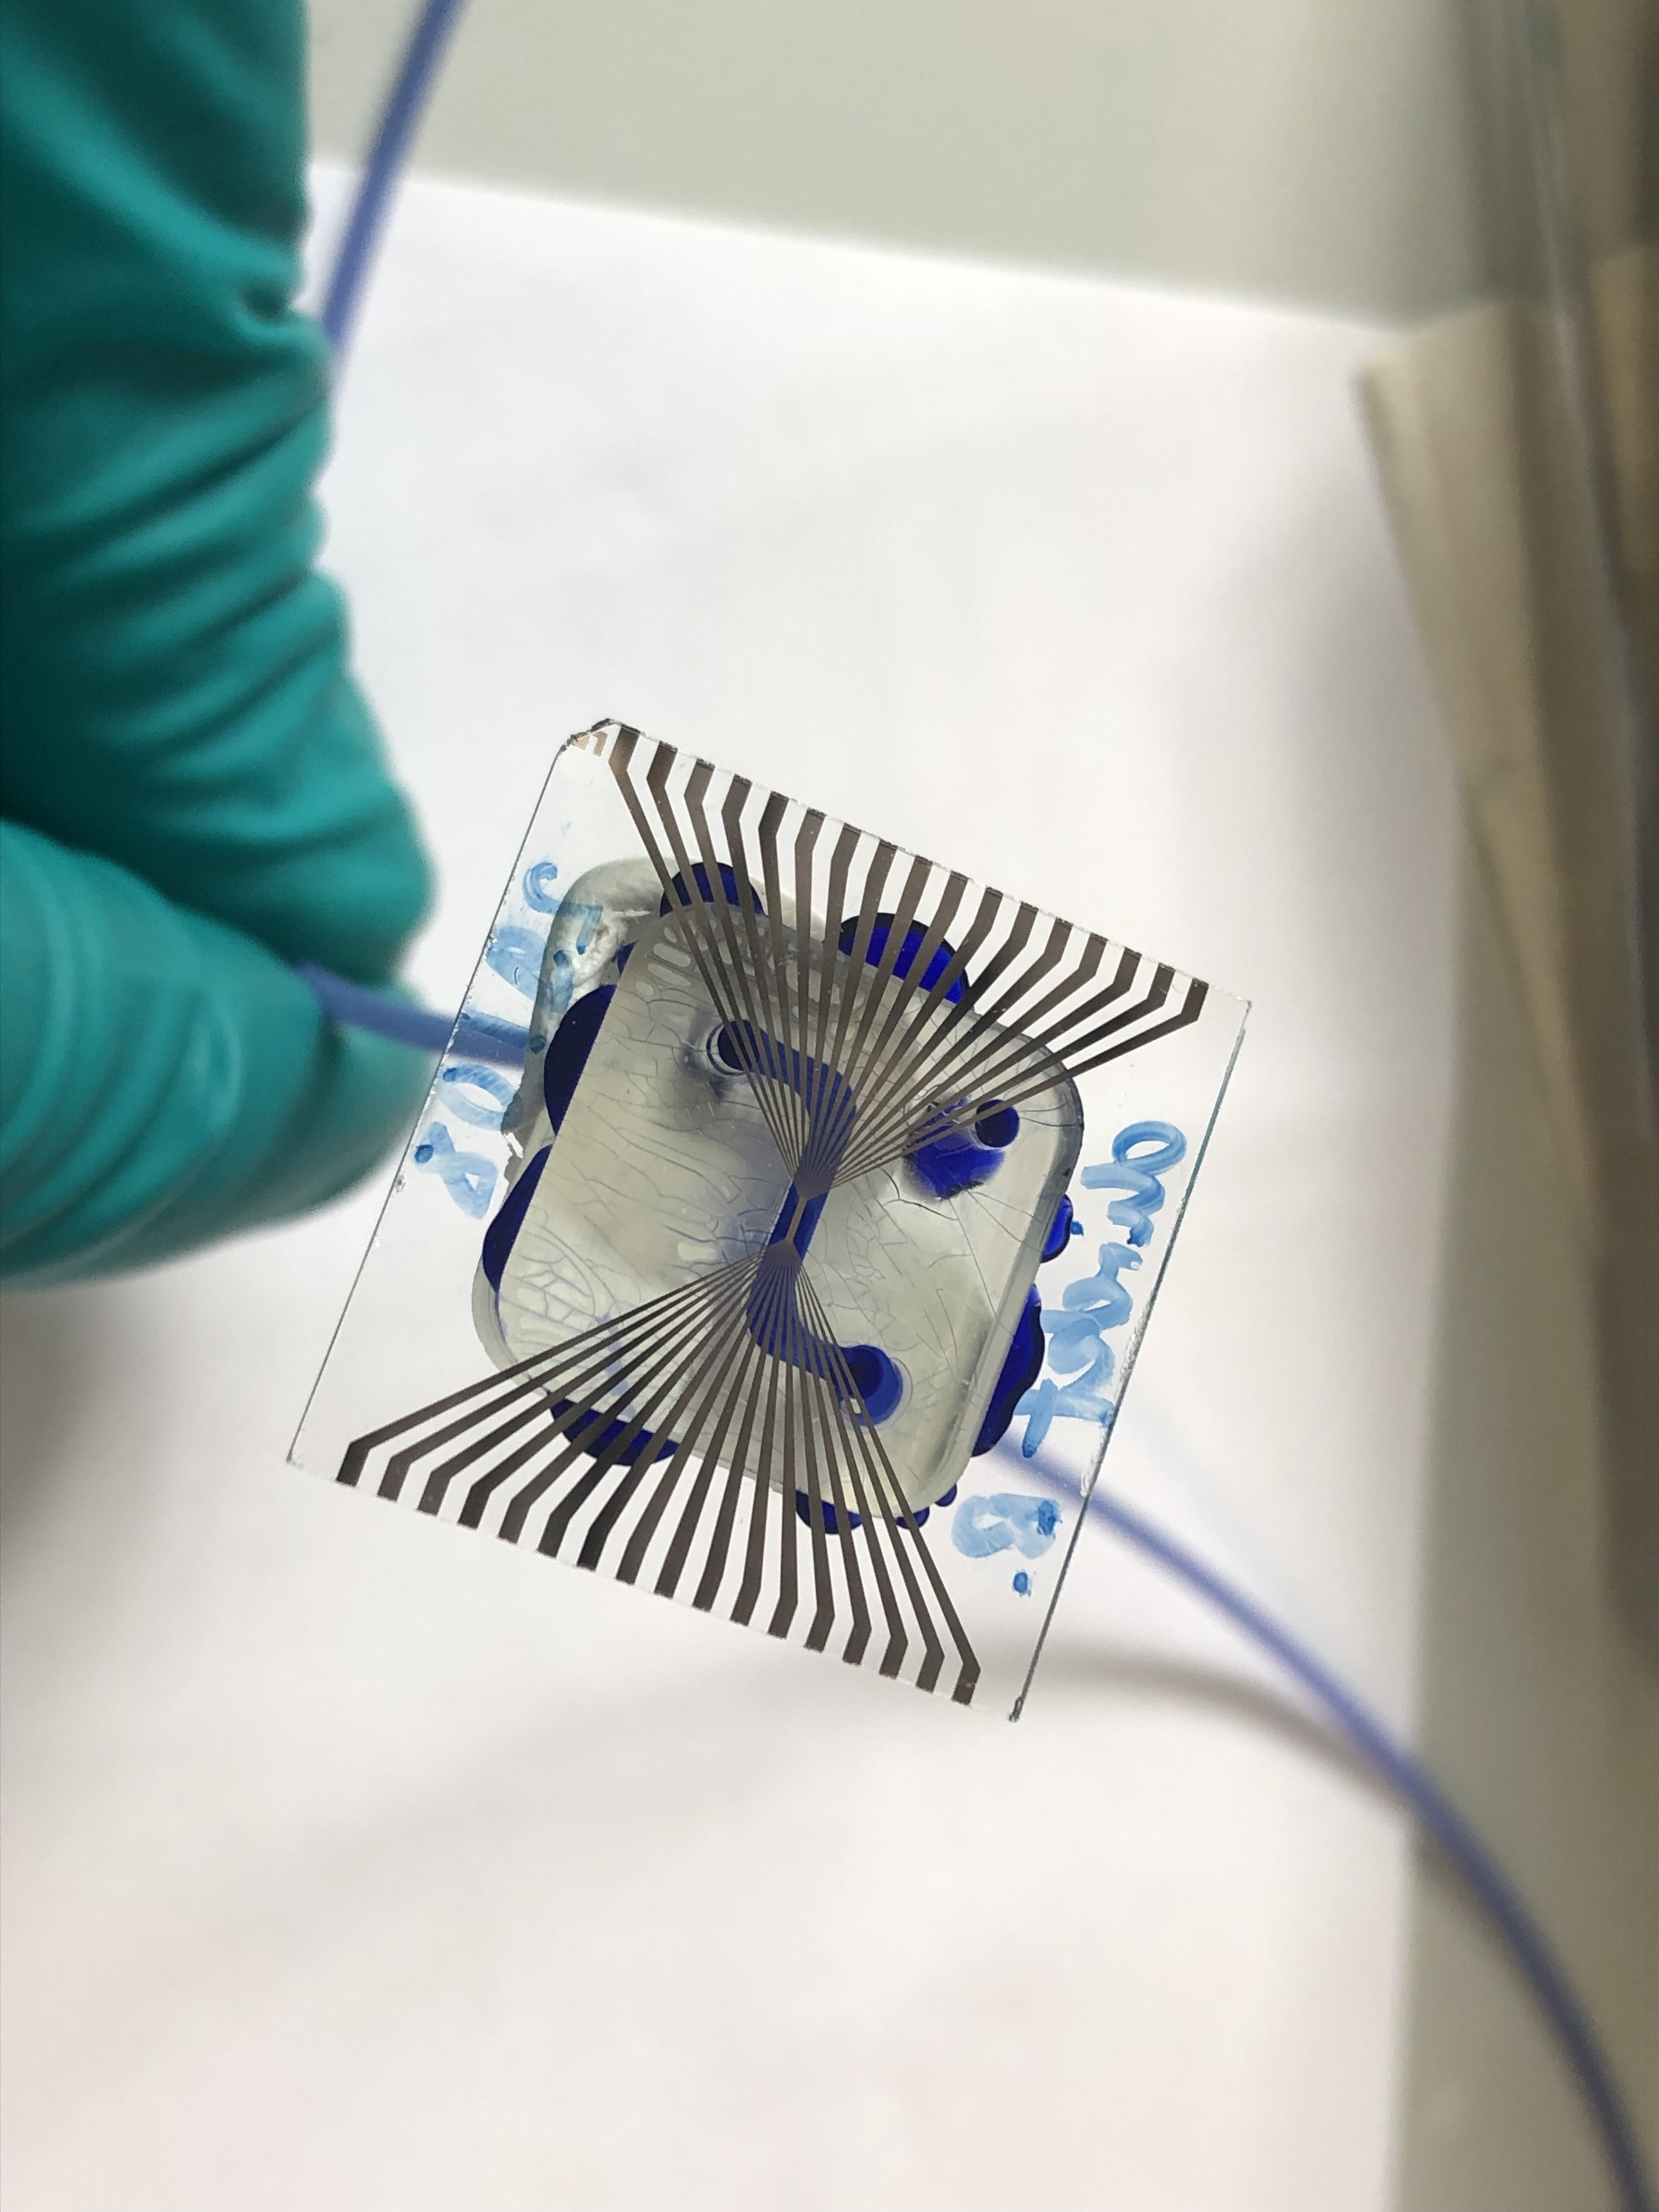
\includegraphics[trim=75 450 100 400mm, clip, width=1.0\textwidth]{img/MIKRORISS.jpeg}
    \caption{Undichte Mikrofluidik auf dem passivierten Sensorchip. Der Kanal wurde zur besseren Sichtbarkeit mit blauer Tinte angefärbt.}
    \label{fig:Mikrofluidik_undicht}
\end{figure}

Als weiterer Ansatz, um die Verbindungsqualität zu erhöhen, wurde ein Plasmacleaning der Werkstücke für \SI{0.7}{\minute} in O$_2$-Plasma - ähnlich zu einer PDMS - Fabrikationsmethode - getestet. Die ersten qualitativen Tests verliefen dahingehend ebenfalls negativ.\\

Ein zusätzlicher Faktor für die mangelnde Druckfestigkeit sind auch Risse an der Unterseite des Drucks. Deren Entstehung konnte im Verlauf des Praktikums nicht abschließend geklärt werden, vermutlich sind jedoch Spannungen innerhalb des Materials durch ungleichmäßige Polymerisation oder Schrumpfung verantwortlich.


\subsection{Elektrochemische Vermessung des Passivierungslayers}
Zusätzlich zu den Verbindungstests mit der Passivierung wurden auch die elektrochemischen Eigenschaften der Elektroden nach der Passivierung durch EIS und CV analysiert. Es wurde erwartet, dass bedeckte Elektroden eine höhere Impedanz und eine kleinere Hysterese im CV besitzen. Außerdem können vollkommen bedeckte Elektroden die charakteristischen Peaks eines Elektrolyten nicht anzeigen.

\begin{figure}[!htb]
\begin{subfigure}[l]{0.49\linewidth}
\centering
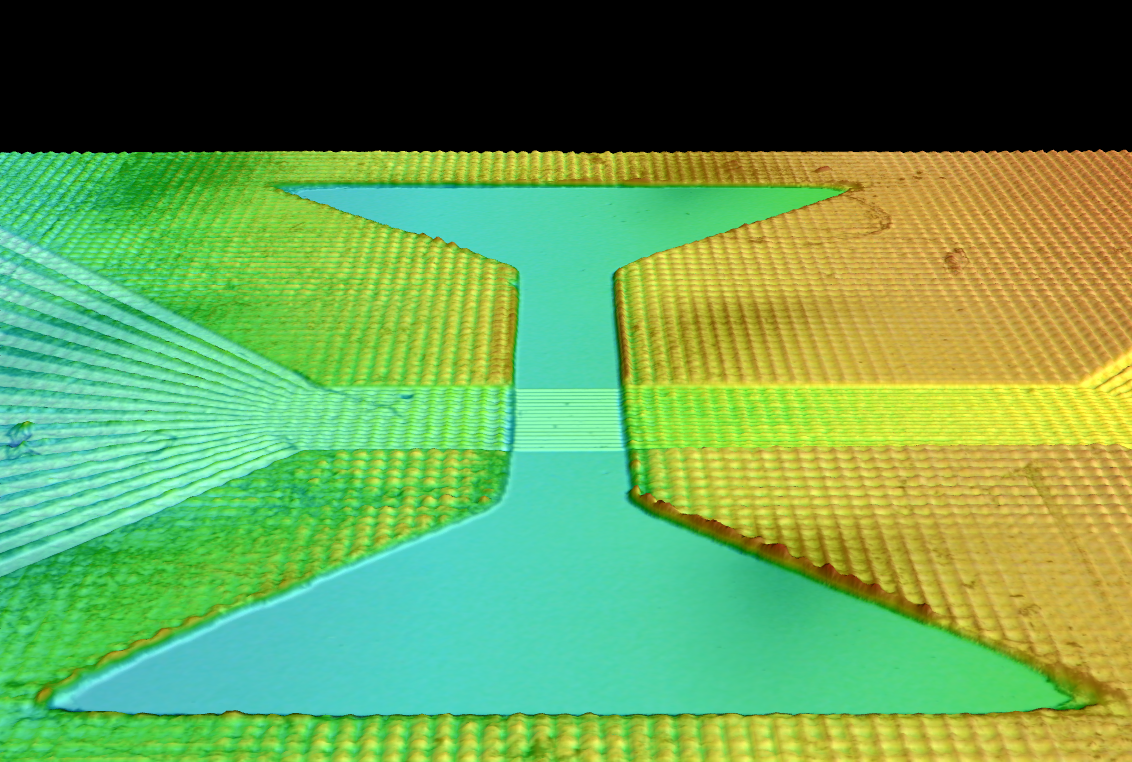
\includegraphics[trim=0 0mm 0 115,clip,width=\linewidth]{img/180mu.png}
\subcaption{\SI{180}{\micro\meter} Passivierung}
\end{subfigure}%
\hspace{6mm}
\begin{subfigure}[r]{0.49\linewidth}
\centering
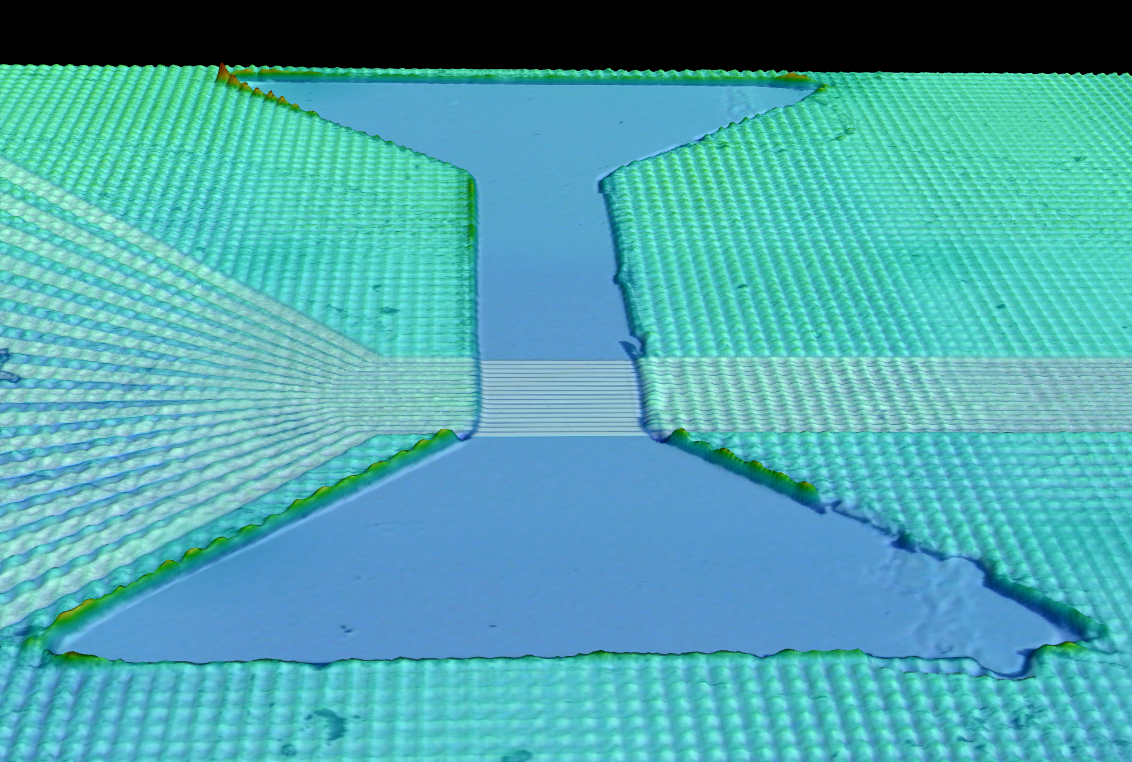
\includegraphics[trim=0 20mm 0 50,clip,width=\linewidth]{img/240um.png}
\subcaption{\SI{240}{\micro\meter} Passivierung}
\end{subfigure}
\caption{Passivierung der Elektrodenstrukturen nach der Behandlung mit \SI{13}{\percent}-iger Schwefelsäure}
\label{fig:passivierung}
\end{figure}

Im Zuge der Experimente wurden Elektrodenöffnungen mit \SIlist{180;210;240}{\micro\meter} Breite vermessen. In den Versuchen wurden CV und EIS der Elektroden vor und nach der Behandlung mit Schwefelsäure gemessen. Während der Reinigung mit 13\% Schwefelsäure, wurden 40 CV-Zyklen mit kurzgeschlossenen Elektroden durchgeführt.


\begin{figure}[!htb]
\begin{subfigure}[l]{0.31\linewidth}
\centering
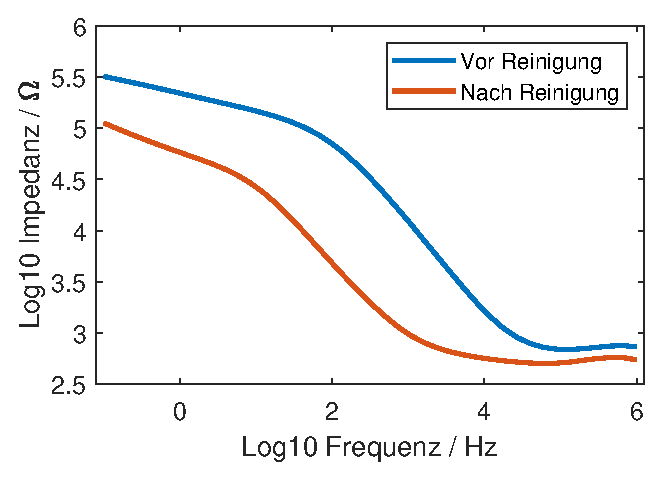
\includegraphics[trim=0 0mm 0 0,clip,width=\linewidth]{plot/EIS_180um.eps}
\subcaption{EIS vor und nach dem Reinigungszyklus}
\label{fig:EIS}
\end{subfigure}%
\hspace{4mm}
\begin{subfigure}[c]{0.31\linewidth}
\centering
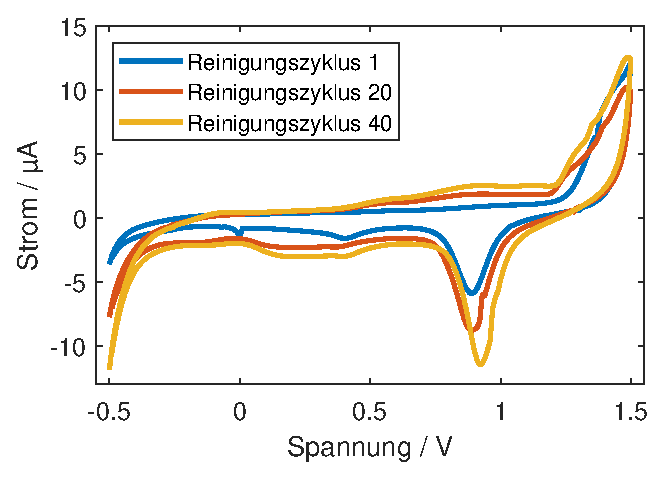
\includegraphics[trim=0 0mm 0 0,clip,width=\linewidth]{plot/Cleaning_180um.eps}
\subcaption{CV-Zyklen während der Elektrodenreinigung}
\label{fig:CV_reinigung}
\end{subfigure}%
\hspace{4mm}
\begin{subfigure}[r]{0.31\linewidth}
\centering
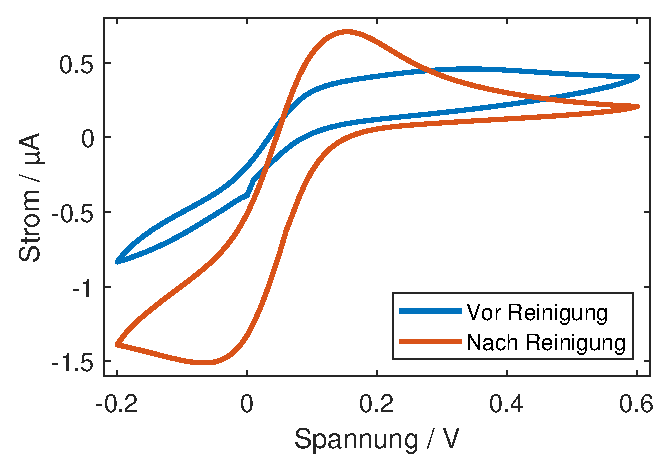
\includegraphics[trim=0 0 0 0,clip,width=\linewidth]{plot/CV_180um.eps}
\subcaption{CV vor und nach dem Reinigungszyklus}
\label{fig:CV}
\end{subfigure}
\caption{Elektrochemische Charakterisierung der Elektrode 13 unter einem Passivierungslayer mit \SI{180}{\micro\meter} Breite}
\label{fig:180um_ElChem}
\end{figure}

Die kurzgeschlossenen Elektroden produzierten im CV einen charakteristischen Peak bei \SI{0.9}{\volt} während der Reinigung. Die Entfernung des Mikrofilms ist außerdem für die Vergrößerung der Hysteresenfläche verantwortlich.(Abb. \ref{fig:CV_reinigung})
Die geringere Impedanz nach der Reinigung (Abb. \ref{fig:EIS}) zeigt zusätlich die Entfernung des vorhandenen Mikrofilms auf den einzelnen Elektrode 13 durch die Schwefelsäure. In einem CV nach der Reinigung (oranger Graph, Abb.\ref{fig:CV}) zeigen sich außerdem im Ansatz charakteristische Peaks in der Hysterese. Die - qualitativ - selben Werte ergeben sich ebenfalls für die Messungen mit Passivierungsstrukturen, die \SIlist{30;60}{\micro\meter} breiter sind.

\subsection{Flussratensensor}
Mit den fertig assemblierten Sensoren aus passiviertem Sensorchip und Mikrofluidik wurde dann versucht durch EIS eine Korrelation der Impedanz zur Flussrate zu finden. Dazu wurden bei unterschiedlichen Drücken Impedanzspektrogramme erstellt und in Matlab ausgewertet. Qualitativ ist ein leichter Trend zu erkennen, der jedoch nicht signifikant ist. 

\begin{figure}[!h]
    \centering
    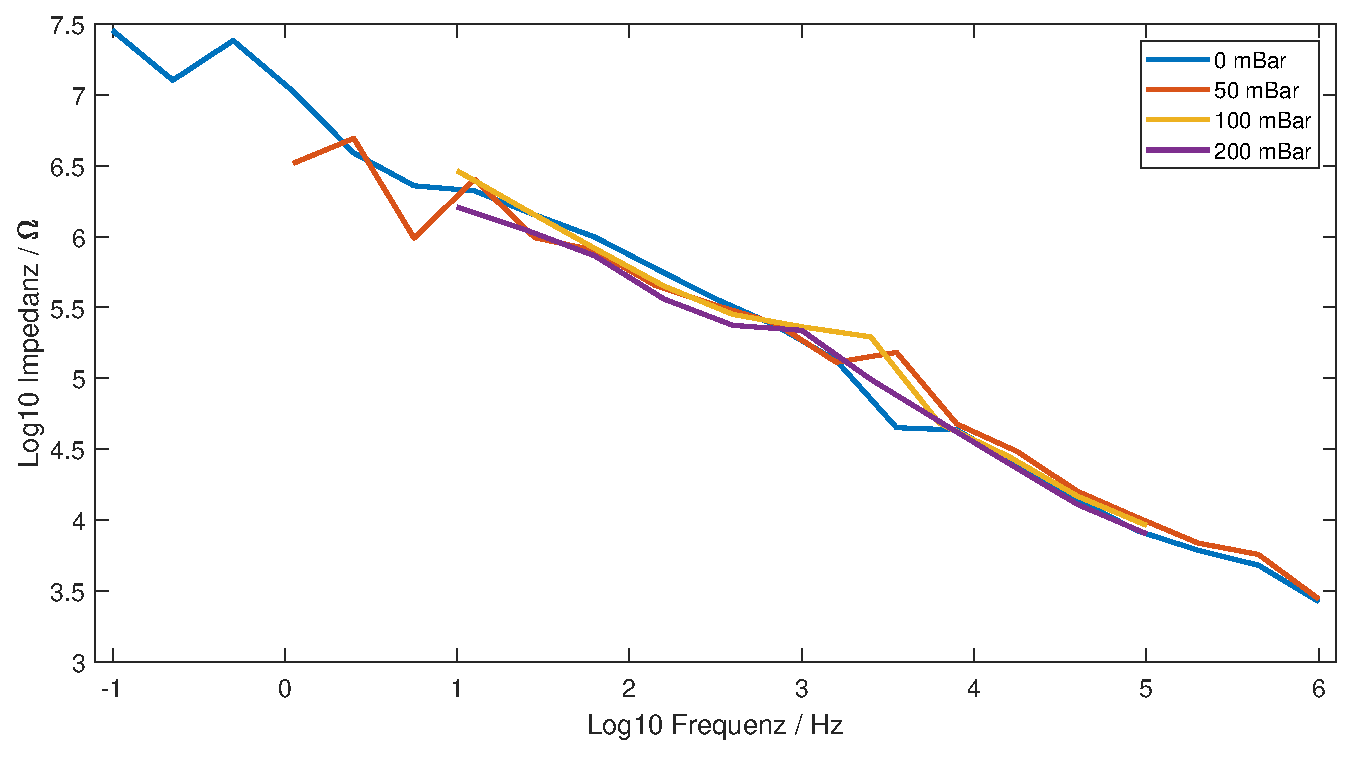
\includegraphics[width=\linewidth]{plot/FlowRate.eps}
    \caption{EIS bei verschiedenen Flussraten von \SI{20}{\milli\Molar} KCl}
    \label{fig:FlowRate}
\end{figure}
\clearpage

\begin{figure}[!h]
    \centering
    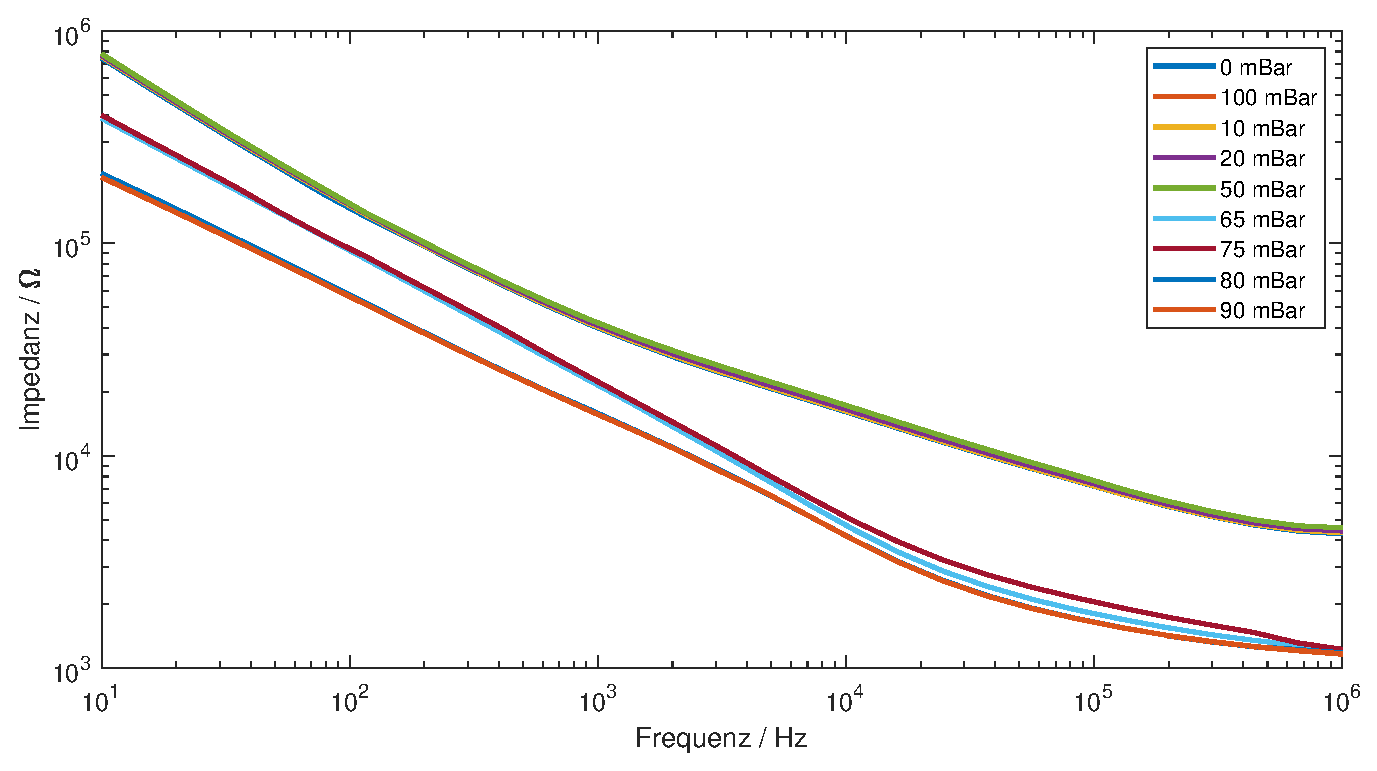
\includegraphics[width=\linewidth]{plot/FlowRate_fine.eps}
    \caption{EIS bei verschiedenen Flussraten von \SI{20}{\milli\Molar} KCl}
    \label{fig:FlowRate_fine}
\end{figure}



 \subsection{3D-Druck der Elektrodenstrukturen}
 Die PVP-AgNP-Elektroden aus dem parallel gelaufenen 3D-Druck wiesen einige Schwachstellen auf.  Auf dem Foto (Abb. \ref{fig:inkjet}) sind bereits einige schwarze Stellen auf den Silberstrukturen sichtbar, an denen die Tinte ungünstig verlaufen ist bzw. gedruckt wurde. Dies lässt sich auf die Oberflächenspannung der Tinte selbst und die Überlappung bzw. den Ausfall einiger Nozzles zurückführen. 
 \begin{figure}[!htb]
     \centering
     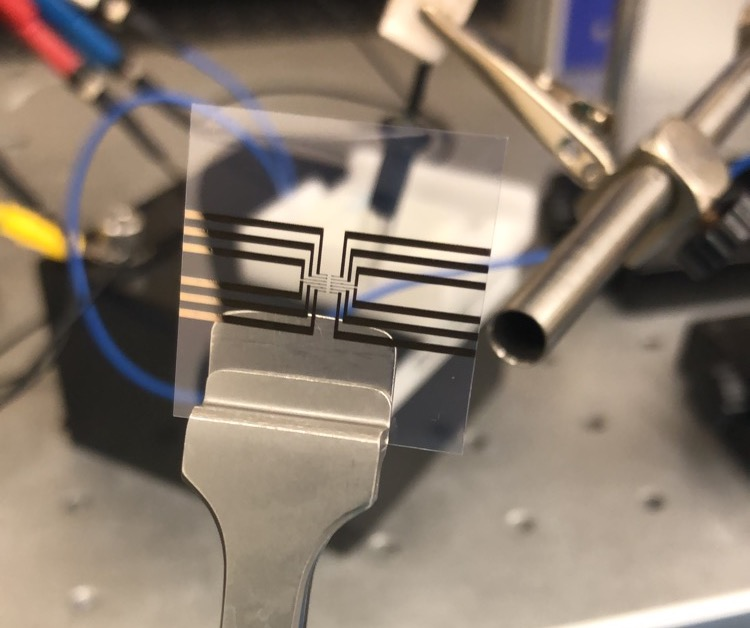
\includegraphics [trim=100 200 200 100,clip,width=.5\linewidth]{img/inkjet_chip.jpeg}
     \caption{Gedruckte Silberelektroden aus dem Inkjet-3D-Drucker.}
     \label{fig:inkjet}
 \end{figure}

\subsection{Galvanisierung der Silberelektroden}
Die fertig prozessierten Silberelektroden wurden nun mit Goldcyanid galvanisiert, um die Cytokompatibilität zu gewährleisten. Nach einigen Ablösungen des Goldes von den Elektroden bzw. einem allgemein schlechten Galvanisierungsergebnis, wurde das  Reduktionspotential von \SI{-1.0}{\volt} auf \SI{-0.9}{\volt} verringert, was zuverlässigere Beschichtungen lieferte.

\subsection{Aerosoldruck der Pillar-Strukturen}
Im Anschluss wurde auf die galvanisierten Elektroden PEDOT:PSS Pillars mittels Aerosol-Jetting gedruckt. Nach der Bestimmung passender Drücke im Scher-, Absaug- und Atomisierungsstrom, wurden auf die Feedlines Pillarstrukturen mit \SI{30}{\micro\meter} Höhe gedruckt.
    
    \clearpage
    \section{Diskussion der Ergebnisse}
    Die in einem Praktikum generierten Ergebnisse bergen einige Unsicherheiten, die sich durch fehlende Gerätekenntnis und mangelnde Erfahrung in speziellen Forschungsgebieten ergeben. Es wurde versucht den menschlichen Fehler durch die Etablierung von Standardverfahren und -prozessen zu minimieren, jedoch lässt sich nicht ausschließen, dass bei manuellen Prozessen einige systematische Fehler gemacht wurden.

Es ist beispielsweise immer noch fraglich, wie sich bei einer geringeren Leistung des SLA eine geringere Tiefe des Kanals - also mehr polymerisiertes Material im Kanal - ergeben kann. Auch die Ergebnisse zum Bonding können durch eine schlechte Silanisierung oder Fehler in einem der anderen Prozesschritte erklärt werden, zumal der Prozess vor dem Praktikum als etabliert galt. 

Aufgrund des kleinen Zeitrahmens konnten auch einige Daten, die durch die Oberflächenvermessung der Teststrukturen zur Druckerauflösung bereits generiert wurden, nicht analysiert werden. Hier sind beispielsweise die um \SI{45}{\degree} gedrehten Kanäle bzw. Wells und die Axondioden zu nennen.

Darüber hinaus steht auch eine definitive Aussage über die Höhe des Mikrofilms auf den Sensorelektroden aus. Die hier verwendeten Messverfahren konnten den Sachverhalt nicht abschließend klären. Als möglicher Beweis könnte das Abkleben der Hälfte eines Glaschips vor der Passivierung dienen. Dadurch könnte man auf einer Seite den Abstand zwischen Passivierung und unbehandelten Elektroden messen, während auf der anderen Seite die üblichen Öffnungen in der Passivierung vermessen werden. Eine andere Möglichkeit könnte eine optische Profilometrie auf Basis der unterschiedlichen Grenzflächeneigenschaften von PEGDA-Glas und Luft-Glas bzw. PEGDA-Gold und Luft-Gold sein.


    
    \clearpage
    \section{Fazit und Ausblick}
    Im Zuge des Praktikums sollten zwei verschiedene Arbeitspakete bearbeitet werden; zum Einen der \textit{Aufbau eine Zellkultursensor-Systems für die Messung von Aktionspotentialen} und zum Anderen das \textit{Prototyping eines impedanz-basierten Flussratensensors}. Grundlegend lässt sich sagen, dass durch die Neuheit der Technologie und der Geräte eine gewisse Einarbeitungszeit erforderlich ist, bevor effektiv und selbstständig an den Geräte gearbeitet werden kann. Daraus resultiert eine geringere Signifikanz und Genauigkeit der früher erworbenen Daten gegenüber der später Gemessenen. 
Darüber hinaus konnten - bedingt durch Gerätausfälle und Wartezeiten - die \SI{8}{\hour} pro Tag nur bedingt effektiv genutzt werden. Als Konsequenz wurden nicht alle Ziele des Praktikums erreicht. 

Während des Praktikums haben wir Evaluationsstrukturen für den SLA designt, in einem festgelegten Parameterraum gedruckt und analysiert. Somit konnten wir einige Auflösungslimits des Druckers bestimmen bzw. validieren. Des Weiteren konnten wir eine simple Mikrofluidik, sowie Schraubverbindungen für Schlauchfittings 3D-drucken und zusammen mit einer optimalen Passivierungsstruktur mechanisch funktionale Flussratensensoren herstellen. Die Analyse dieser konnte aus Zeitgründen nur teilweise erstellt werden. Das Bonding der Passivierung mit der Mikrofluidik ist immernoch ein sehr unzuverlässig funktionierender Prozess, der weiterer Optimierung bedarf.

Das Zellkultursensor-Projekt wurde nach dem Inkjet-Druck der Elektroden durch einen Defekt am Drucker ausgebremst. So konnten die Silberstrukturen noch mit einem optimierten Galvanisierungsprozess beschichtet werden, dann aber das Proktoll nicht weitergeführt werden. Als Workaround konnten wir die Pillarstrukturen noch mit Aerosol-Jet-Technologie auf die Feedlines drucken. Mangels Zeit konnten aber weder eine 3D-Zellkulturkammer, noch die optimalen Axondioden evaluiert und dementsprechend kein funktionaler Sensor gebaut werden.

Zusammenfassend lässt sich also festhalten, dass zwar nur ein Teil der angepeilten Ziele erreicht wurde, jedoch einige wichtige Erkenntnisse generiert und Prozesse optimiert wurden. Außerdem können auf Basis der erhaltenen Resultate neue Experimente besser geplant bzw. deren Ausgänge besser eingeschätzt werden. Nicht zuletzt ist der Lernerfolg sowohl im Bereich der 3D-Drucktechnologie, als auch der (Elektro-)chemie eine wertvolle Errungenschaft des Praktikums.
    
    \clearpage
    \section{Ergänzende Datenauswertungen}
\label{appendix}

\begin{figure}[!htb]
    \centering
    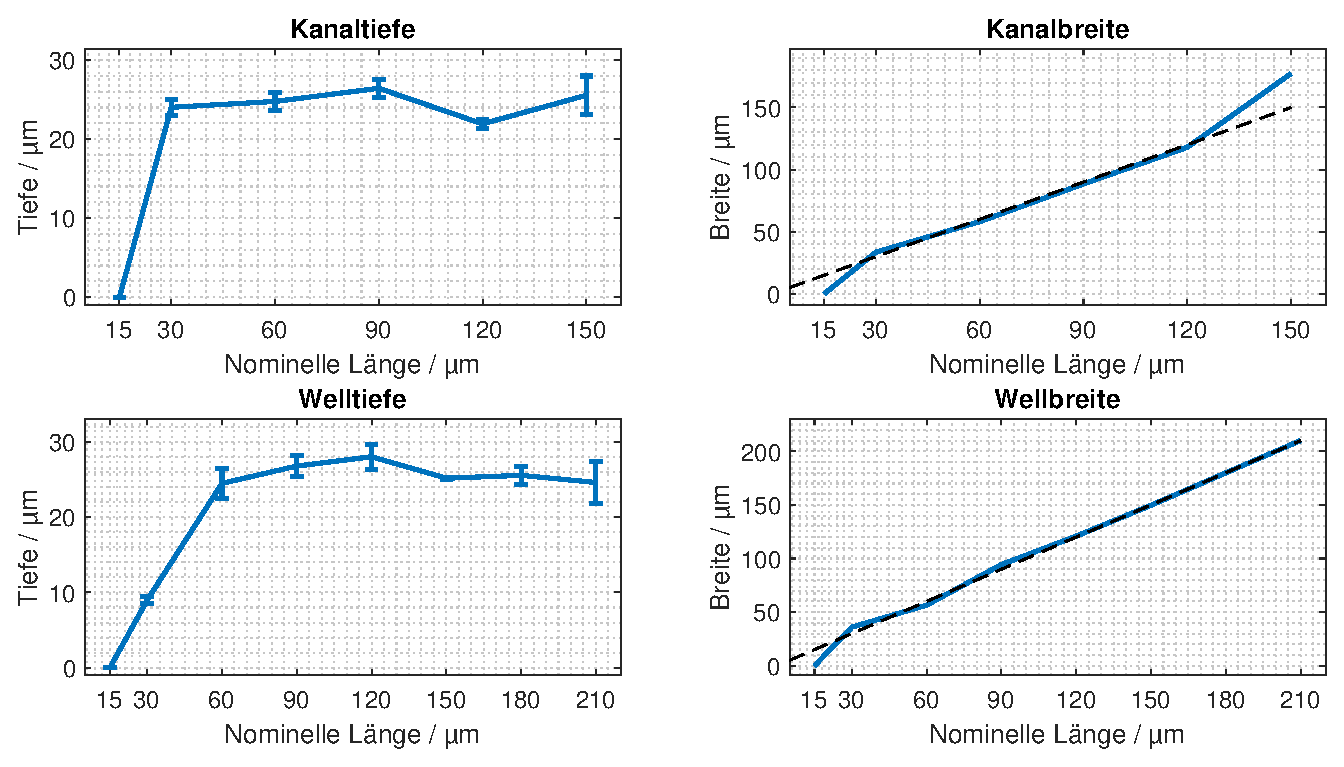
\includegraphics[width=\linewidth]{plot/25um_SL_ResolutionV1.eps}
    \caption{Profilometrie des \SI{25}{\micro\meter}-Einzellayers aus MPC.}
    \label{fig:MPC_25um}
\end{figure}


\begin{figure}[!htb]
    \centering
    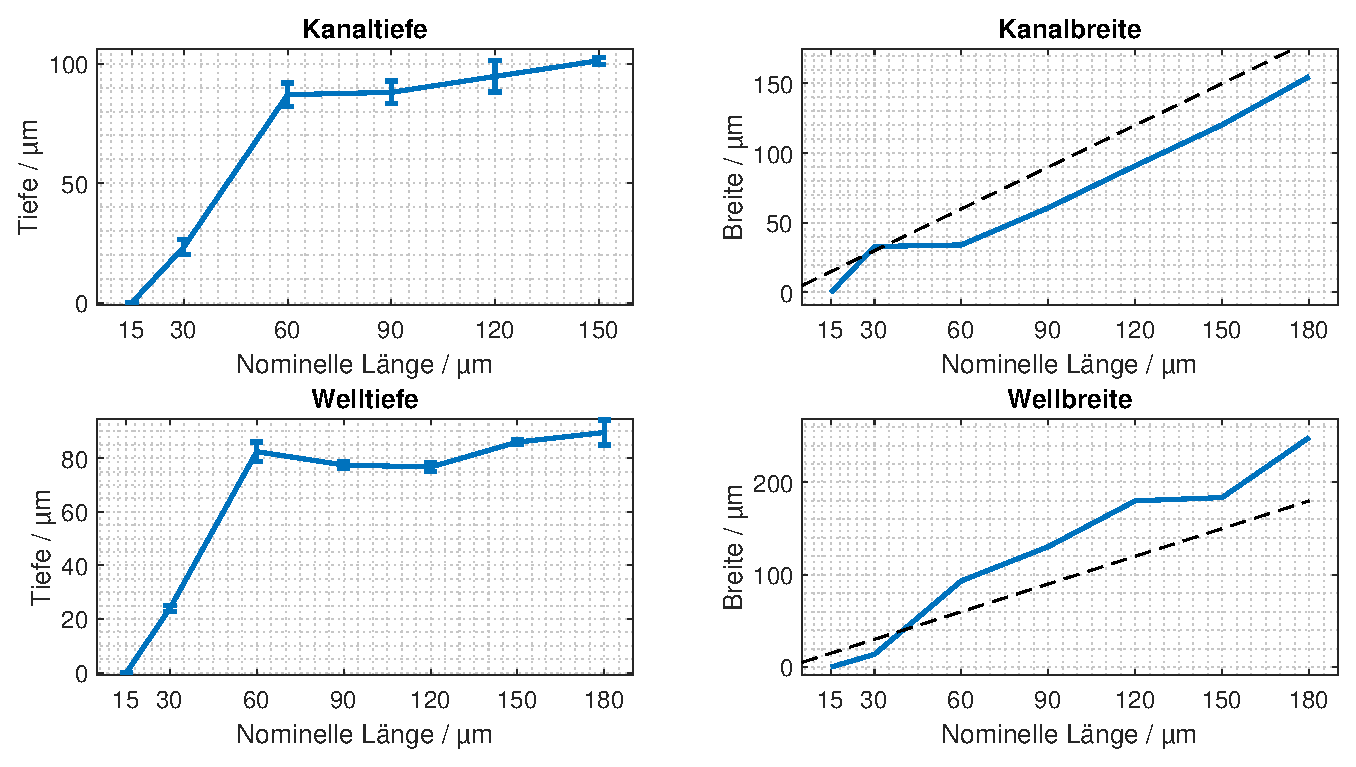
\includegraphics[width=\linewidth]{plot/100um_SL_ResolutionV1.eps}
    \caption{Profilometrie des \SI{100}{\micro\meter}-Einzellayers aus MPC.}
    \label{fig:MPC_100um}
\end{figure}

\begin{figure}[!htb]
    \centering
    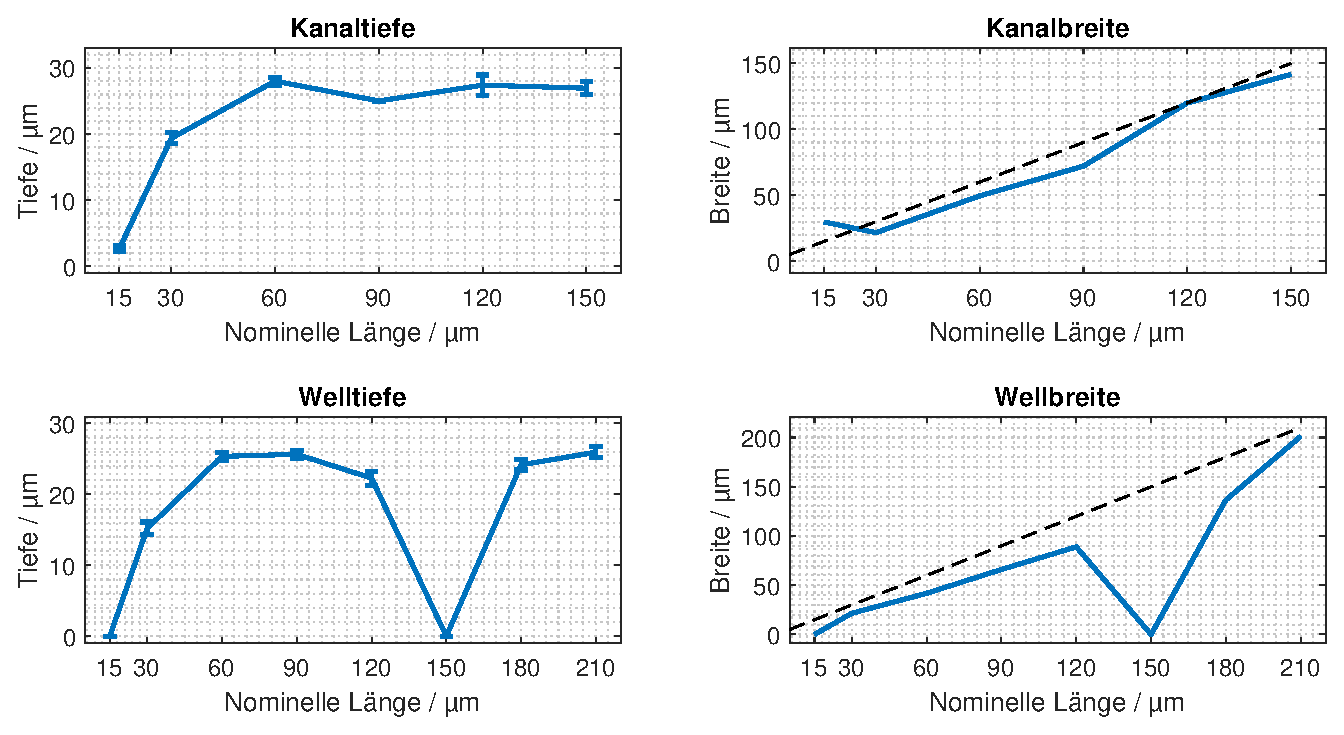
\includegraphics[width=\linewidth]{plot/PEGDA_25um_SL_ResolutionV1.eps}
    \caption{Profilometrie des \SI{25}{\micro\meter}-Einzellayers aus PEGDA.}
    \label{fig:PEGDA_25um}
\end{figure}

\begin{figure}[!htb]
    \centering
    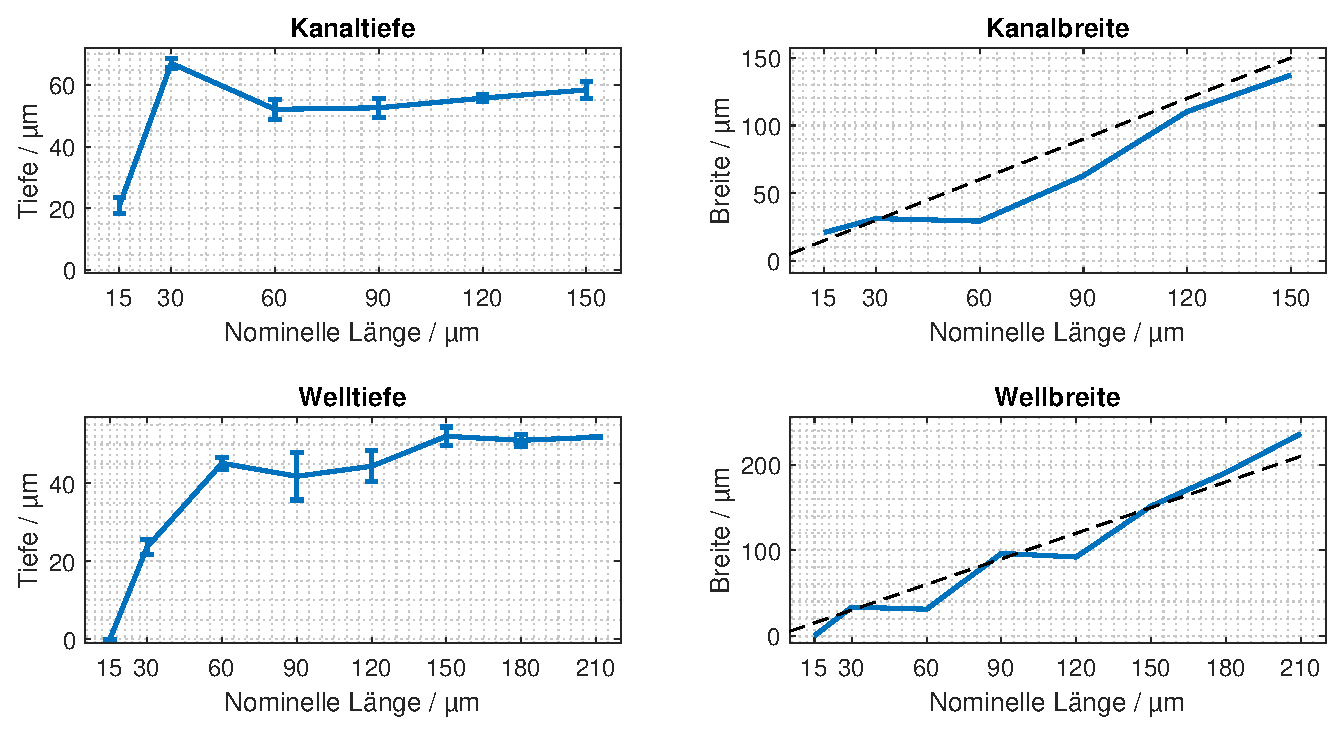
\includegraphics[width=\linewidth]{plot/PEGDA_50um_SL_ResolutionV1.eps}
    \caption{Profilometrie des \SI{50}{\micro\meter}-Einzellayers aus PEGDA.}
    \label{fig:PEGDA_50um}
\end{figure}

    \clearpage
\bibliographystyle{unsrtnat}
\bibliography{literature.bib}

\clearpage
\listoffigures


\end{document}
